 \documentclass{vkr}
\usepackage[english, russian]{babel} % переносы
\usepackage{graphicx} % для вставки картинок
\graphicspath{{images/}} % путь к изображениям
\usepackage[hidelinks]{hyperref}
\usepackage{float} % определяет метод H для рисунка с переносом на следующую страницу, ели не помещается
\usepackage{pdflscape}
\addto{\captionsrussian}{\renewcommand{\refname}{СПИСОК ИСПОЛЬЗОВАННЫХ ИСТОЧНИКОВ}}
\usepackage{xltabular} % для вставки таблиц
\usepackage{makecell}
\renewcommand\theadfont{} % шрифт в /thead
\usepackage{array} % для определения новых типов столбцов таблиц
\newcolumntype{T}{>{\centering\arraybackslash}X} % новый тип столбца T - автоматическая ширина столбца с выравниванием по центру
\newcolumntype{R}{>{\raggedleft\arraybackslash}X} % новый тип столбца R - автоматическая ширина столбца с выравниванием по правому краю
\newcolumntype{C}[1]{>{\centering\let\newline\\\arraybackslash\hspace{0pt}}m{#1}} % новый тип столбца C - фиксированная ширина столбца с выравниванием по центру
\newcolumntype{r}[1]{>{\raggedleft\arraybackslash}p{#1}} % новый тип столбца r - фиксированная ширина столбца с выравниванием по правому краю
\newcommand{\centrow}{\centering\arraybackslash} % командой \centrow можно центрировать одну ячейку (заголовок) в столбце типа X или p, оставив в оcтальных ячейках другой тип выравнивания
\newcommand{\finishhead}{\endhead\hline\endlastfoot}
\newcommand{\continuecaption}[1]{\captionsetup{labelformat=empty} \caption[]{#1}\\ \hline }
\usepackage{etoolbox}
\AtBeginEnvironment{xltabular}{\refstepcounter{tablecnt}} % подсчет таблиц xltabular, обычные таблицы подсчитываются в классе

\usepackage[tableposition=top]{caption} % подпись таблицы вверху
\captionsetup{strut=off}
\setlength{\intextsep}{0pt} % Vertical space above & below [h] floats
\setlength{\textfloatsep}{0pt} % Vertical space below (above) [t] ([b]) floats
\DeclareCaptionLabelFormat{gostfigure}{Рисунок #2} %подпись рисунка
\DeclareCaptionLabelFormat{gosttable}{Таблица #2} %подпись таблицы
\DeclareCaptionLabelSeparator{gost}{~--~} %разделитель в рисунках и таблицах
\captionsetup{labelsep=gost}
\captionsetup[figure]{aboveskip=10pt,belowskip=4mm,justification=centering,labelformat=gostfigure} % настройка подписи рисунка
\captionsetup[table]{font={stretch=1.41},skip=0pt,belowskip=0pt,aboveskip=8.5pt,singlelinecheck=off,labelformat=gosttable} % настройка подписи таблицы

\setlength{\LTpre}{8mm} % отступ сверху таблицы
\setlength{\LTpost}{6mm} % отступ снизу таблицы

\usepackage{enumitem}
\setlist{nolistsep,wide=\parindent,itemindent=*} % отступы вокруг списков, выравнивание с учетом разделителя

\usepackage{color} %% это для отображения цвета в коде
\usepackage{listings} %% листинги кода
\setmonofont[Scale=0.7]{Verdana} % моноширный шрифт для листинга

\definecolor{codegreen}{rgb}{0,0.6,0}
\definecolor{codegray}{rgb}{0.5,0.5,0.5}
\definecolor{codepurple}{rgb}{0.58,0,0.82}

\lstset{ %
language=C,                 % выбор языка для подсветки (здесь это С)
numbers=left,               % где поставить нумерацию строк (слева\справа)
numberstyle=\tiny,           % размер шрифта для номеров строк
stepnumber=1,                   % размер шага между двумя номерами строк
numbersep=5pt,                % как далеко отстоят номера строк от подсвечиваемого кода
commentstyle=\color{codegreen},
keywordstyle=\color{magenta},
numberstyle=\tiny\color{codegray},
stringstyle=\color{codepurple},
basicstyle=\linespread{0.95}\ttfamily,
backgroundcolor=\color{white}, % цвет фона подсветки - используем \usepackage{color}
showspaces=false,            % показывать или нет пробелы специальными отступами
showstringspaces=false,      % показывать или нет пробелы в строках
showtabs=false,             % показывать или нет табуляцию в строках
frame=single,              % рисовать рамку вокруг кода
tabsize=2,                 % размер табуляции по умолчанию равен 2 пробелам
captionpos=t,              % позиция заголовка вверху [t] или внизу [b] 
breaklines=true,           % автоматически переносить строки (да\нет)
breakatwhitespace=false, % переносить строки только если есть пробел
escapeinside={\%*}{*)}   % если нужно добавить комментарии в коде
}

\makeatletter % чтобы допускались русские комментарии в листингах
\lst@InputCatcodes
\def\lst@DefEC{%
 \lst@CCECUse \lst@ProcessLetter
  ^^80^^81^^82^^83^^84^^85^^86^^87^^88^^89^^8a^^8b^^8c^^8d^^8e^^8f%
  ^^90^^91^^92^^93^^94^^95^^96^^97^^98^^99^^9a^^9b^^9c^^9d^^9e^^9f%
  ^^a0^^a1^^a2^^a3^^a4^^a5^^a6^^a7^^a8^^a9^^aa^^ab^^ac^^ad^^ae^^af%
  ^^b0^^b1^^b2^^b3^^b4^^b5^^b6^^b7^^b8^^b9^^ba^^bb^^bc^^bd^^be^^bf%
  ^^c0^^c1^^c2^^c3^^c4^^c5^^c6^^c7^^c8^^c9^^ca^^cb^^cc^^cd^^ce^^cf%
  ^^d0^^d1^^d2^^d3^^d4^^d5^^d6^^d7^^d8^^d9^^da^^db^^dc^^dd^^de^^df%
  ^^e0^^e1^^e2^^e3^^e4^^e5^^e6^^e7^^e8^^e9^^ea^^eb^^ec^^ed^^ee^^ef%
  ^^f0^^f1^^f2^^f3^^f4^^f5^^f6^^f7^^f8^^f9^^fa^^fb^^fc^^fd^^fe^^ff%
  ^^^^20ac^^^^0153^^^^0152%
  % Basic Cyrillic alphabet coverage
  ^^^^0410^^^^0411^^^^0412^^^^0413^^^^0414^^^^0415^^^^0416^^^^0417%
  ^^^^0418^^^^0419^^^^041a^^^^041b^^^^041c^^^^041d^^^^041e^^^^041f%
  ^^^^0420^^^^0421^^^^0422^^^^0423^^^^0424^^^^0425^^^^0426^^^^0427%
  ^^^^0428^^^^0429^^^^042a^^^^042b^^^^042c^^^^042d^^^^042e^^^^042f%
  ^^^^0430^^^^0431^^^^0432^^^^0433^^^^0434^^^^0435^^^^0436^^^^0437%
  ^^^^0438^^^^0439^^^^043a^^^^043b^^^^043c^^^^043d^^^^043e^^^^043f%
  ^^^^0440^^^^0441^^^^0442^^^^0443^^^^0444^^^^0445^^^^0446^^^^0447%
  ^^^^0448^^^^0449^^^^044a^^^^044b^^^^044c^^^^044d^^^^044e^^^^044f%
  ^^^^0401^^^^0451%
  %%%
  ^^00}
\lst@RestoreCatcodes
\makeatother


% Режим шаблона (должен быть включен один из трех)
%\ВКРtrue
\Практикаtrue
%\Курсоваяtrue

\newcommand{\Дисциплина}{<<Проектирование и архитектура программных систем>>} % для курсовой
\newcommand{\КодСпециальности}{09.03.04} % Курсовая
\newcommand{\Специальность}{Программная инженерия} % Курсовая
\newcommand{\Тема}{Система тестирования} % ВКР Курсовая
\newcommand{\ТемаВтораяСтрока}{}
\newcommand{\ГдеПроводитсяПрактика}{ООО <<МЦОБ Онлайн-сервисы>>} % для практики
\newcommand{\РуководительПрактПредпр}{Чаплыгин А. А.} % для практики
\newcommand{\ДолжнРуководительПрактПредпр}{директор} % для практики
\newcommand{\РуководительПрактУнивер}{Чаплыгин А. А.} % для практики
\newcommand{\ДолжнРуководительПрактУнивер}{к.т.н. доцент} % для практики
\newcommand{\Автор}{Н. Г. Коваль}
\newcommand{\АвторРод}{Коваля Н. Г.}
\newcommand{\АвторПолностьюРод}{Коваля Никиты Георгиевича} % для практики
\newcommand{\Шифр}{21-06-0117}
\newcommand{\Курс}{4} % для практики
\newcommand{\Группа}{ПО-11б}
\newcommand{\Руководитель}{А. А. Чаплыгин} % для ВКР и курсовой
\newcommand{\Нормоконтроль}{А. А. Чаплыгин} % для ВКР
\newcommand{\ЗавКаф}{А. В. Малышев} % для ВКР
\newcommand{\ДатаПриказа}{«07» апреля 2023~г.} % для ВКР
\newcommand{\НомерПриказа}{1505-с} % для ВКР
\newcommand{\СрокПредоставления}{«24» июня 2024~г.} % для ВКР, курсового

\begin{document}
\maketitle
\ifПрактика{}\else{
   \newpage
\begin{center}
\large\textbf{Минобрнауки России}

\large\textbf{Юго-Западный государственный университет}
\vskip 1em
\normalsize{Кафедра программной инженерии}
\vskip 1em
\ifВКР{
        \begin{flushright}
        \begin{tabular}{p{.4\textwidth}}
        \centrow УТВЕРЖДАЮ: \\
        \centrow Заведующий кафедрой \\
        \hrulefill \\
        \setarstrut{\footnotesize}
        \centrow\footnotesize{(подпись, инициалы, фамилия)}\\
        \restorearstrut
        «\underline{\hspace{1cm}}»
        \underline{\hspace{3cm}}
        20\underline{\hspace{1cm}} г.\\
        \end{tabular}
        \end{flushright}
        }\fi
\end{center}
\vspace{1em}
  \begin{center}
  \large
\ifВКР{
ЗАДАНИЕ НА ВЫПУСКНУЮ КВАЛИФИКАЦИОННУЮ РАБОТУ
  ПО ПРОГРАММЕ БАКАЛАВРИАТА}
  \else
ЗАДАНИЕ НА КУРСОВУЮ РАБОТУ (ПРОЕКТ)
\fi
\normalsize
  \end{center}
\vspace{1em}
{\parindent0pt
  Студента \АвторРод, шифр\ \Шифр, группа \Группа
  
1. Тема «\Тема\ \ТемаВтораяСтрока»
\ifВКР{
утверждена приказом ректора ЮЗГУ от \ДатаПриказа\ № \НомерПриказа
}\fi.

2. Срок предоставления работы к защите \СрокПредоставления

3. Исходные данные для создания программной системы:

3.1. Перечень решаемых задач:}

\renewcommand\labelenumi{\theenumi)}

\begin{enumerate}
\item проанализировать структуру системы тестирования;
\item  разработать концептуальную модель системы редактирования и прохождения тестов;
\item спроектировать программную систему редактирования и прохождения тестов;
\item сконструировать и протестировать программную систему редактирования и прохождения тестов.
\end{enumerate}

{\parindent0pt
  3.2. Входные данные и требуемые результаты для программы:}

\begin{enumerate}
\item Входными данными для программной системы являются: текстовые данные вопросов, типов вопросов и ответов на них, введённые пользователем или загруженные из файла.
\item Выходными данными для программной системы являются: сформированные вопросы и соответствующий их типам интерфейс; сформированные ответы на
данные вопросы; сведения о результатах прохождения тестов пользователями
\end{enumerate}

{\parindent0pt

  4. Содержание работы (по разделам):
  
  4.1. Введение
  
  4.1. Анализ предметной области
  
4.2. Техническое задание: основание для разработки, назначение разработки,
требования к программной системе, требования к оформлению документации.

4.3. Технический проект: общие сведения о программной системе, проект
данных программной системы, проектирование архитектуры программной системы, проектирование пользовательского интерфейса программной системы.

4.4. Рабочий проект: спецификация компонентов и классов программной системы, тестирование программной системы, сборка компонентов программной системы.

4.5. Заключение

4.6. Список использованных источников

5. Перечень графического материала:

\списокПлакатов

\vskip 2em
\begin{tabular}{p{6.8cm}C{3.8cm}C{4.8cm}}
Руководитель \ifВКР{ВКР}\else работы (проекта) \fi & \lhrulefill{\fill} & \fillcenter\Руководитель\\
\setarstrut{\footnotesize}
& \footnotesize{(подпись, дата)} & \footnotesize{(инициалы, фамилия)}\\
\restorearstrut
Задание принял к исполнению & \lhrulefill{\fill} & \fillcenter\Автор\\
\setarstrut{\footnotesize}
& \footnotesize{(подпись, дата)} & \footnotesize{(инициалы, фамилия)}\\
\restorearstrut
\end{tabular}
}

\renewcommand\labelenumi{\theenumi.}

   \abstract{РЕФЕРАТ}

Объем работы равен \formbytotal{lastpage}{страниц}{е}{ам}{ам}. Работа содержит \formbytotal{figurecnt}{иллюстраци}{ю}{и}{й}, \formbytotal{tablecnt}{таблиц}{у}{ы}{}, \arabic{bibcount} библиографических источников и \formbytotal{числоПлакатов}{лист}{}{а}{ов} графического материала. Количество приложений – 2. Графический материал представлен в приложении А. Фрагменты исходного кода представлены в приложении Б.

Перечень ключевых слов: коммерческий сайт, Система, CMS, Битрикс, Joomla, аддитивные технологии, 3D-принтеры, услуги, сервисы, информатизация, автоматизация, информационные технологии, веб-форма,  Apache, классы, база данных, средства защиты информации, подсистема, компонент, модуль, сущность, информационный блок, метод, контент-редактор, администратор, пользователь, web-сайт.

Объектом разработки является web-сайт компании,  занимающейся производством 3D-принтеров, выпуском оборудования для создания порошков, разработкой программного обеспечения и организацией центров аддитивного производства.

Целью выпускной квалификационной работы является привлечение клиентов, увеличение заказов, информирование о продукции и услугах путем создания сайта компании.

В процессе создания сайта были выделены основные сущности путем создания информационных блоков, использованы классы и методы модулей, обеспечивающие работу с сущностями предметной области, а также корректную работу web-сайта, разработаны разделы, содержащие информацию о компании, ее деятельности, производимой продукции и услугах, разработан сервис по заказу 3D-деталей.

При разработке сайта использовалась система управления контентом "<1С-Битрикс: Управление сайтом">.

Разработанный сайт был успешно внедрен в компании.

\selectlanguage{english}
\abstract{ABSTRACT}
  
The volume of work is \formbytotal{lastpage}{page}{}{s}{s}. The work contains \formbytotal{figurecnt}{illustration}{}{s}{s}, \formbytotal{tablecnt}{table}{}{s}{s}, \arabic{bibcount} bibliographic sources and \formbytotal{числоПлакатов}{sheet}{}{s}{s} of graphic material. The number of applications is 2. The graphic material is presented in annex A. The layout of the site, including the connection of components, is presented in annex B.

List of keywords: commercial website, System, CMS, Bitrix, Joomla, additive technologies, 3D printers, services, services, informatization, automation, information technology, web form, Apache, classes, database, component, module, entity, information block, method, content editor, administrator, user, web site.

The object of the research is the analysis of information technologies for the development of a production company's website.

The object of the development is the website of a company engaged in the production of 3D printers, the production of equipment for the creation of powders, software development and the organization of additive manufacturing centers.

The purpose of the final qualifying work is to attract customers, increase orders, inform about products and services by creating a company website.

In the process of creating the site, the main entities were identified by creating information blocks, classes and methods of modules were used to ensure work with the entities of the subject area, as well as the correct operation of the website, sections containing information about the company, its activities, products and services were developed, a service for ordering 3D parts was developed.

When developing the site, the content management system <<1C – Bitrix: Site Management>> was used.

The developed website was successfully implemented in the company.
\selectlanguage{russian}
}\fi
\tableofcontents
\section*{ОБОЗНАЧЕНИЯ И СОКРАЩЕНИЯ}

JSON — текстовый формат обмена данными, основанный на JavaScript.

Сериализация — это процесс преобразования объекта в поток байтов для сохранения или передачи в память, базу данных или файл.

Десериализация - это процесс преобразования данных, сериализованных в определенном формате, обратно в объекты или структуры данных, которые они представляют.

ИС -- информационная система.

ИТ -- информационные технологии. 

КТС -- комплекс технических средств.

ОМТС -- отдел материально-технического снабжения. 

ПО -- программное обеспечение.

РП -- рабочий проект.

ТЗ -- техническое задание.

ТП -- технический проект.

UML (Unified Modelling Language) -- язык графического описания для объектного моделирования в области разработки программного обеспечения.

\ifПрактика{}\else{% !TeX spellcheck = ru_RU-Russian
\section*{ВВЕДЕНИЕ}
\addcontentsline{toc}{section}{ВВЕДЕНИЕ}

В современном образовательном процессе, где акцент делается на индивидуальном подходе и непрерывном обучении, системы для оценки и контроля знаний играют ключевую роль. Они представляют собой мощный инструмент для автоматизации оценки уровня знаний, умений и навыков обучающихся, предоставляя объективную и оперативную обратную связь.

Эффективная система тестирования знаний заменяет традиционные методы контроля и трансформирует сам процесс обучения, позволяя преподавателям оперативно выявлять пробелы в знаниях, корректировать учебные планы и предлагать индивидуальные траектории обучения. Студенты, в свою очередь, получают возможность оценивать свой прогресс, выявлять свои сильные и слабые стороны и фокусироваться на областях, требующих дополнительного внимания.

Система тестирования уровня знаний предназначена для оценки знаний и навыков учащихся, студентов или сотрудников в определенной области. Она позволяет оценить уровень подготовленности людей и выявить их сильные и слабые стороны. Такая система может не только проверить знания, но и определить необходимость дальнейшего обучения или повышения квалификации, а также помогает контролировать уровень достижений и прогресса в обучении.

\emph{Цель настоящей работы} – разработка программно-информационной системы, позволяющей создавать тесты, осуществлять тестирование пользователей, осуществлять сбор и анализ результатов тестирования. Для достижения поставленной цели необходимо решить \emph{следующие задачи:}
\begin{itemize}
\item провести анализ предметной области;
\item разработать концептуальную модель программно-информационной системы для оценки и контроля знаний;
\item спроектировать программно-информационную систему для оценки и контроля знаний;
\item реализовать программно-информационную систему для оценки и контроля знаний средствами графических библиотек.
\end{itemize}

\emph{Структура и объем работы.} Отчет состоит из введения, 4 разделов основной части, заключения, списка использованных источников, 2 приложений. Текст выпускной квалификационной работы равен \formbytotal{lastpage}{страниц}{е}{ам}{ам}.

\emph{Во введении} сформулирована цель работы, поставлены задачи разработки, описана структура работы, приведено краткое содержание каждого из разделов.

\emph{В первом разделе} на стадии описания технической характеристики предметной области приводится информация о целях и задачах систем тестирования знаний, а также её классификация и основные компоненты.

\emph{Во втором разделе} на стадии технического задания приводятся требования к разрабатываемому приложению.

\emph{В третьем разделе} на стадии технического проектирования представлены проектные решения для приложения.

\emph{В четвертом разделе} приводится список классов и их методов, использованных при разработке приложения, производится тестирование разработанного приложения.

В заключении излагаются основные результаты работы, полученные в ходе разработки.

В приложении А представлен графический материал.
В приложении Б представлены фрагменты исходного кода. 
}\fi
\section{Анализ предметной области}
\subsection{Характеристика предприятия и его деятельности. Тест длинного заголовка, не должен содержать переносы}

Системы управления тестированием используются для хранения информации о том, как должным образом проводить тестирование, осуществление очередности проведения тестирования в соответствии с его планом, а также для получения информации в виде отчетов о стадии тестирования и качестве тестируемого продукта. Инструменты имеют различные подходы к тестированию и, таким образом, включают в себя различные наборы функций. Обычно они используются для планирования ручного тестирования, сбора данных о результатах прохождения чек-листов и тест-кейсов, а также для получения оперативной информации в виде отчетов. Системы управления тестированием помогают оптимизировать процесс тестирования и обеспечивают быстрый доступ к анализу данных, средствам совместной работы и более качественному взаимодействию между несколькими проектными группами. Многие системы управления тестированием включают в себя возможность работы с требованиями.

Инструменты управления тестированием дают командам возможность консолидировать и структурировать процесс тестирования с помощью одной из систем управления тестированием вместо установки нескольких приложений, которые предназначены для управления только одним процессом или его частью. Некоторые приложения включают передовые инструментальные панели для тщательного отслеживания ключевых показателей, что позволяет легко получать необходимую информацию о стадиях процесса тестирования и качестве тестируемого продукта.

После старта тестирования проекта члены команды могут взаимодействовать через одну из систем управления тестирования путём создания тест-кейсов, чек-листов, назначая ответственных за прохождение их лиц, что упрощает и улучшает качество взаимодействия лиц, проводящих тестирование в рамках конкретного проекта. При создании или прохождении тестов и чек-листов пользователи могут получить доступ к различным функциям систем управления тестированием, которые автоматизируют данную деятельность и благотворно влияют на скорость и качество её выполнения.

\subsection{Система тестирования, их классификация}

В настоящее время определено, что педагогические тесты помогают
получить более объективные оценки уровня знаний, умений, навыков,
проверить соответствие требований к подготовке выпускников вузов заданным
стандартам, выявить пробелы в подготовке персонала.

Тест – это инструмент, состоящий из квалиметрически выверенной системы тестовых заданий, стандартизированной процедуры проведения и заранее спроектированной технологии обработки и анализа результатов, предназначенной для измерения качеств и свойств личности, изменение которых возможно в процессе систематического обучения. Или тест – краткое стандартизированное испытание, допускающее количественную оценку результатов на основе их
статистической обработки. Отбор структура заданий теста зависит от того, какие показатели и факторы интересуют исследователя данной группы лиц. Каждое из заданий теста по своей сути представляет для испытуемого вопрос, проблему. Ответ на вопрос – это всегда устранение некоторых сомнений, колебаний, неопределенности в рассматриваемой ситуации с целью получения новых, более точных знаний.

С точки зрения целей применения можно выделить:

тесты достижений;

критериально-ориентированные тесты, позволяющие сопоставить
уровень индивидуальных учебных достижений с полным объемом знаний,
умений и навыков;

нормативно-ориентированные тесты, сравнивающие испытуемых по
уровню их учебных достижений;

аттестационные тесты, определяющие степень обученности;

тесты прогнозирования результатов обучения по выбранной
технологии обучения.
% !TeX spellcheck = ru_RU-Russian
% !TeX encoding = UTF-8
\section{Техническое задание}
\subsection{Основание для разработки}

Полное наименование системы: «Программно-информационная система для оценки и контроля знаний».
Основанием для разработки программы является задание на выпускную квалификационную работу.

\subsection{Цель и назначение разработки}

Программно-информационная система предназначена для контроля и оценки знаний обучающихся с целью улучшения процесса обучения.

Задачами данной разработки являются:
\begin{enumerate}
\item Создание модуля для создания новых тестов.
\item Создание модуля для создания вопросов.
\item Создание модуля для редактирования вопросов.
\item Создание модуля для авторизации.
\item Создание модуля для регистрации.
\item Создание модуля для просмотра результатов пройденных тестов.
\item Создание модуля для управления пользователями.
\item Создание модуля для пользователя.
\item Создание модуля для администратора.
\item Реализация системы оценивания по результатам теста.
\item Реализация системы хранения тестов и результатов тестов.
\end{enumerate}

\subsection{Требования к данным программной системы}

Входными данными для системы являются:
\begin{itemize}
    \item данные имеющихся тестов;
    \item данные о зарегистрированных пользователях;
    \item ответы на вопросы теста;
    \item данные администратора.
\end{itemize}

Выходными данными для системы являются:
\begin{itemize}
	\item графическое отображение вопросов тестов;
	\item данные создании/изменении тестов;
	\item данные о новых зарегистрированных/добавленных администратором пользователях;
	\item данные о изменении паролей пользователей;
	\item данные результатов пройденных тестов.
\end{itemize}

\subsection{Функциональные требования к программной системе}

В разрабатываемой программно-информационной системе должно
быть предусмотрено наличие два класса пользователей: пользователь и администратор.

Пользователю должны быть доступны следующие функции программы:
\begin{enumerate}
	\item Авторизация.
	\item Регистрация.
	\item Прохождение выбранного теста.
	\item Просмотр собственных результатов пройденных тестов.
\end{enumerate}

Администратору должны быть доступны следующие функции программы:
\begin{enumerate}
	\item Авторизация.
	\item Изменение пароля администратора.
	\item Прохождение выбранного теста.
	\item Просмотр результатов всех пользователей.
	\item Управление пользователями.
	\item Создание новых тестов.
	\item Редактирование имеющихся тестов.
\end{enumerate}

\subsection{Моделирование вариантов использования}

Для разрабатываемой системы тестирования знаний была реализована модель, которая обеспечивает наглядное представление вариантов использования системы.

Она помогает в физической разработке и детальном анализе взаимосвязей объектов.

Диаграмма вариантов описывает функциональное назначение разрабатываемой системы. То есть это то, что система будет непосредственно делать в процессе своего функционирования. Она является исходным концептуальным представлением системы в процессе ее проектирования и разработки. Проектируемая система представляется в виде ряда прецедентов, предоставляемых системой актерам или сущностям, которые взаимодействуют с системой. Актером или действующим лицом является сущность, взаимодействующая с системой извне (например, человек, техническое устройство). Прецедент служит для описания набора действий, которые система предоставляет актеру.

\clearpage

На рисунке ~\ref{user_precedent_diagram:image} в виде диаграммы прецедентов представлены функциональные требования к системе, доступные для пользователя.

\begin{figure}[H]
	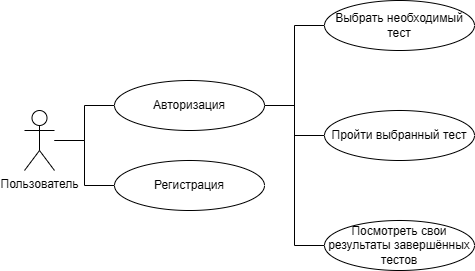
\includegraphics[width=1\linewidth]{диаграмма_прецедентов_пользователь}
	\caption{Диаграмма прецедентов пользователя}
	\label{user_precedent_diagram:image}
\end{figure}

\clearpage

На рисунке ~\ref{admin_precedent_diagram:image} представлены дополнительные функциональные требования к системе для администратора.

\begin{figure}[H]
	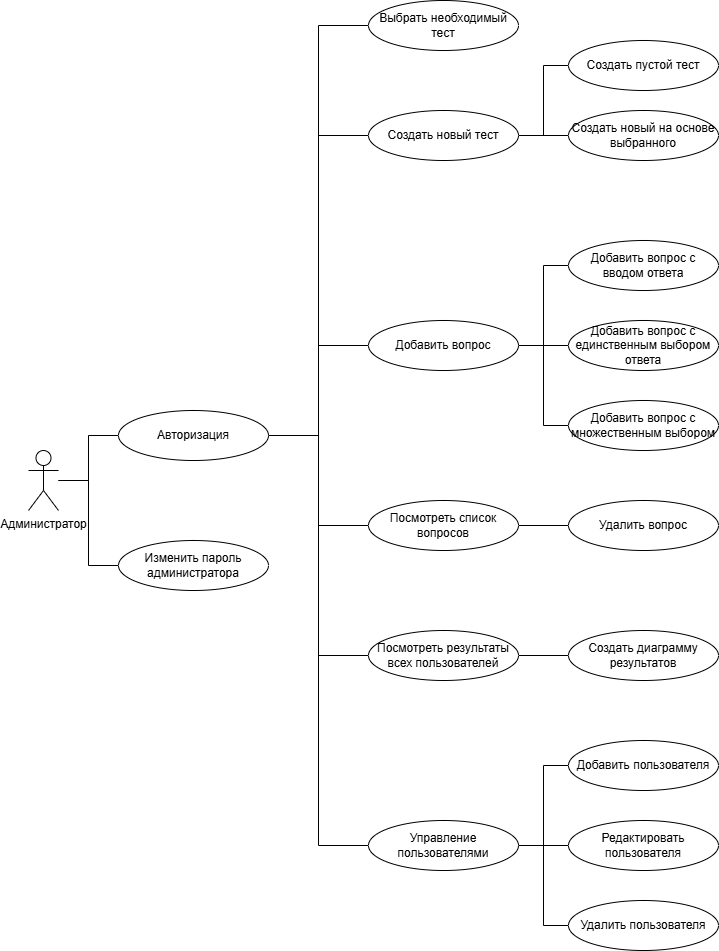
\includegraphics[width=1\linewidth]{диаграмма_прецедентов_администратор}
	\caption{Диаграмма прецедентов администратора}
	\label{admin_precedent_diagram:image}
\end{figure}

На основании анализа предметной области в программе должны быть реализованы следующие варианты использования: 
Для пользователя:
\begin{enumerate}
\item ВИ "<Авторизация">. Данный прецедент позволяет пользователю авторизоваться.
\item ВИ "<Регистрация">. Данный прецедент позволяет зарегистрироваться.
\item ВИ "<Выбрать желаемый тест">. Данный прецедент позволяет пользователю выбрать желаемый тест.
\item ВИ "<Пройти выбранный тест">. Данный прецедент позволяет пользователю приступить к прохождению выбранного теста.
\item ВИ "<Добавить вопрос">. Данный прецедент позволяет пользователю добавить вопрос в выбранном тесте.
\item ВИ "<Удалить вопрос">. Данный прецедент позволяет пользователю удалить вопрос в выбранном тесте.
\item ВИ "<Просмотреть результаты">. Данный прецедент позволяет пользователю посмотреть собственные результаты пройденных тестов.
\item ВИ "<Создать новый тест">. Данный прецедент позволяет пользователю создать новый тест.
\end{enumerate}

Для администратора:
\begin{enumerate}
	\item ВИ "<Авторизоваться как администратор">. Данный прецедент позволяет авторизоваться как администратор и получить соответствующие права.
	\item ВИ "<Изменить пароль администратор">. Данный прецедент позволяет изменить пароль администратор. Требуется ввести старый пароль и два раза повторить новый.
	\item ВИ "<Выбрать желаемый тест">. Данный прецедент позволяет администратору выбрать желаемый тест.
	\item ВИ "<Пройти выбранный тест">. Данный прецедент позволяет администратору приступить к прохождению выбранного теста.
	\item ВИ "<Добавить вопрос">. Данный прецедент позволяет администратору добавить вопрос в выбранном тесте. Возможно добавить три варианта вопроса: с вводом ответа, с единственным выбором из имеющихся ответов, с множественным выбором из имеющихся ответов.
	\item ВИ "<Просмотреть набор выбранного теста">. Данный прецедент позволяет администратору посмотреть состав теста.
	\item ВИ "<Удалить вопрос">. Данный прецедент позволяет администратору удалить выбранный вопрос.
	\item ВИ "<Просмотреть результаты">. Данный прецедент позволяет администратору посмотреть результаты пройденных тестов всех пользователей.
	\item ВИ "<Создать новый тест">. Данный прецедент позволяет администратору создать новый тест. Можно создать пустой тест или копировать текущий набор выбранного теста.
	\item ВИ "<Управление пользователями">. Данный прецедент позволяет администратору добавить нового пользователя, удалить или редактировать уже существующего.
\end{enumerate}

\subsubsection{Описание вариантов использования}

Данные варианта использования <<Пройти выбранный тест>>.

Входными данными является выбранный тест, имя пользователя.

Выходными данными прецедента <<Пройти выбранный тест>> являются вопросы с ответами и результат прохождения теста.

Основной исполнитель: Пользователь.

Заинтересованные лица и их требования: Пользователь хочет пройти тест.

Предусловие: поля для ввода имени, ответа на вопрос должны быть заполнены.

Постусловие: приложение проверит введены ли данные, если нет, сообщит об этом пользователю.

Основной успешный сценарий:
\begin{enumerate}
	\item Пользователь запускает программу.
	\item Пользователь проходит авторизацию, введя своё имя.
	\item Пользователь попадает в меню.
	\item Пользователь выбирает желаемый тест.
	\item Пользователь нажимает кнопку <<Пройти тест>>.
	\item Пользователь попадает в окно теста.
	\item Пользователь выбирает или вводит ответы.
	\item Пользователь по окончании теста видит его результат.
	\item Пользователь закрывает приложение.
\end{enumerate}

Данные варианта использования <<Создать новый тест>>.

Входными данными является пароль администратора, данные для нового теста.

Выходными данными прецедента <<Создать новый тест>> являются новый тест с вопросами и ответами.

Основной исполнитель: Администратор.

Заинтересованные лица и их требования: Администратор хочет создать тест и добавить в него вопрос

Предусловие: поля для ввода пароля администратора, текста вопроса и его ответа должны быть заполнены.

Постусловие: приложение проверит введены ли данные, если нет, сообщит об этом администратору.

Основной успешный сценарий:
\begin{enumerate}
	\item Администратор запускает программу.
	\item Администратор проходит авторизацию, введя пароль.
	\item Администратор попадает в меню.
	\item Администратор нажимает кнопку <<Создать тест>>.
	\item Администратор попадает в окно создания теста.
	\item Администратор нажимает кнопку <<Создать новый тест>>.
	\item Администратор нажимает кнопку <<Вернуться в меню>>.
	\item Администратор попадает в меню.
	\item Администратор нажимает кнопку <<Добавить вопрос>>.
	\item Администратор попадает в меню добавления вопроса.
	\item Администратор нажимает кнопку добавить базовый вопрос.
	\item Администратор в окне создания базового вопроса вводит текст и ответ вопроса.
	\item Администратор нажимает кнопку добавить вопрос.
	\item Администратор закрывает приложение.
\end{enumerate}

\paragraph{Вариант использования <<Регистрация>>}

Заинтересованные лица и их требования: пользователь желает зарегистрироваться в приложении.
\newline Предусловие: открыто окно "<Авторизация пользователя">.
\newline Постусловие: создаётся аккаунт нового пользователя на основании введённых данных для регистрации, имени и пароля.
\newline Основной успешный сценарий:
\begin{enumerate}
	\item Пользователь переходит в окно "<Регистрация">.
	\item Приложение отображает соответствующее окно регистрации с полями для ввода имени и пароля (см. рисунок ~\ref{reg_window:image}).
	\item Пользователь заполняет текстовые поля "<Имя"> и "<Пароль"> (см. рисунок ~\ref{reg_data:image}). Данные поля обязательны для заполнения. Имя должно состоять только из символов без цифр, минимум два символа. Имя должно быть уникальным.
	\item Пользователь нажимает кнопку "<Зарегистрироваться">.
	\item Приложение проверяет введённые пользователем имя и пароль. Если данные некорректны, сообщает об этом пользователю. При корректных данных приложение создаёт новый аккаунт и сообщает пользователю об успешной регистрации (см. рисунок ~\ref{successful_reg:image}).
\end{enumerate}

\newpage
\begin{figure}[ht]
	\centering
	
\includegraphics[width=0.5\linewidth]{регистрация.png}
	\caption{Окно "<Регистрация">}
	\label{reg_window:image}
\end{figure}
\begin{figure}[ht]
	\centering
	\includegraphics[width=0.5\linewidth]{регистрация_данные.png}
	\caption{Ввод имени и пароля в окне "<Регистрация">}
	\label{reg_data:image}
\end{figure}
\begin{figure}[ht]
	\centering
	
\includegraphics[width=0.5\linewidth]{успешная_регистрация.png}
	\caption{Уведомление об успешной регистрации}
	\label{successful_reg:image}
\end{figure}

\paragraph{Вариант использования <<Авторизация пользователя>>}

Заинтересованные лица и их требования: пользователь желает авторизоваться в приложении.
\newline Предусловие: открыто окно "<Авторизация пользователя">.
\newline Постусловие: авторизация произведена, отображается окно "<Меню пользователя">.
\newline Основной успешный сценарий:
\begin{enumerate}
	\item Пользователь переходит в окно "<Авторизация пользователя"> (см. рисунок ~\ref{user_auth_window:image}).
	\item Приложение отображает соответствующее окно авторизации с полями для ввода имени и пароля.
	\item Пользователь заполняет текстовые поля "<Имя"> и "<Пароль"> (см. рисунок ~\ref{user_auth_data:image}). Данные поля обязательны для заполнения.
	\item Пользователь нажимает кнопку "<Перейти в меню">.
	\item Приложение проверяет введённые пользователем имя и пароль. Если данные некорректны, сообщает об этом пользователю. При корректных данных приложение закрывает текущее окно авторизации и открывает окно "<Меню пользователя"> (см. рисунок ~\ref{user_menu_1:image}).
\end{enumerate}

\begin{figure}[H]
	\centering
	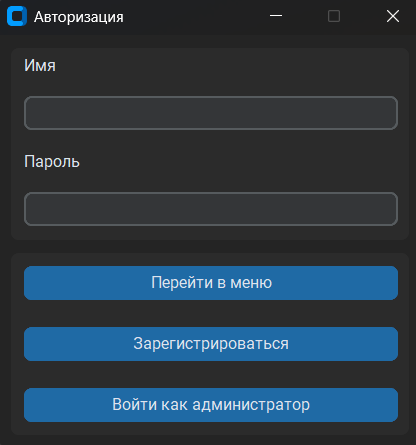
\includegraphics[width=0.6\linewidth]{окно_авторизации_пользователя.png}
	\caption{Окно "<Авторизация пользователя">}
	\label{user_auth_window:image}
\end{figure}
\begin{figure}[H]
	\centering
	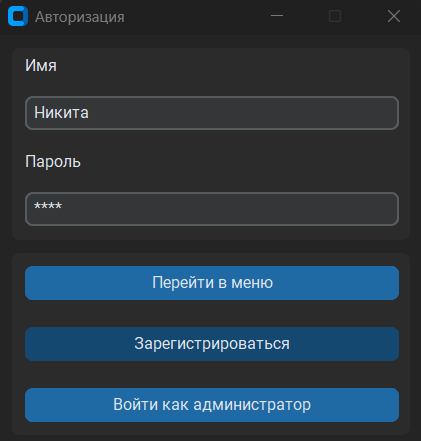
\includegraphics[width=0.6\linewidth]{авторизация_пользователя_данные.png}
	\caption{Ввод имени и пароля пользователя}
	\label{user_auth_data:image}
\end{figure}
\begin{figure}[H]
	\centering
	
\includegraphics[width=1\linewidth]{меню_п_1.png}
	\caption{Окно "<Меню пользователя">}
	\label{user_menu_1:image}
\end{figure}

\paragraph{Вариант использования <<Тестирование>>}

Заинтересованные лица и их требования: пользователь желает пройти тестирование.
\newline Предусловие: открыто окно "<Меню пользователя"> или "<Меню администратора">.
\newline Постусловие: Даны ответы на все вопросы, приложение отображает результаты тестирования пользователю и сохраняет отчёт результатов.
\newline Основной успешный сценарий:
\begin{enumerate}
	\item Пользователь выбирает желаемый тест в меню с помощью выпадающего списка и нажимает кнопку "<Начать тест"> (см. рисунок ~\ref{user_menu_window:image}).
	\item Приложение отображает окно теста и выводит текст первого вопроса (см. рисунок ~\ref{test_window:image}). Отображение вопроса зависит от его типа: для вопроса с вводом ответа будет создано поле для ввода; для вопроса с единственным выбором ответа будут созданы кнопки с ответам, только одну можно выбрать для ответа; для вопроса с множественным выбором будут созданы кнопки с ответами, можно выбрать сразу несколько ответов.
	\item Пользователь отвечает на вопрос и нажимает кнопку "<Ответить">.
	\item Приложение проверяет ответ пользователя и выводит следующий вопрос. 
	\item Когда пользователь отвечает на последний вопрос, приложение выводит результат прохождения теста и сохраняет его.
\end{enumerate}

\newpage
\begin{figure}[ht]
	\centering
	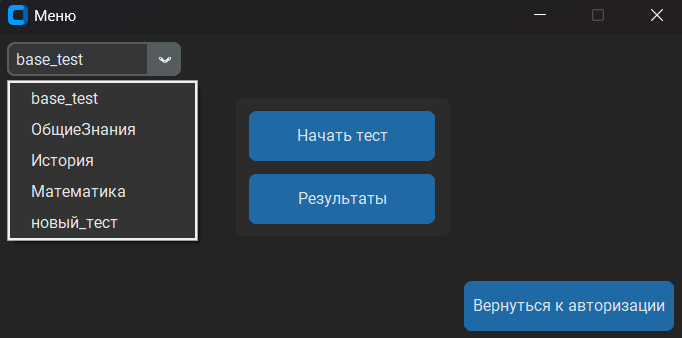
\includegraphics[width=1\linewidth]{меню_пользователя.png}
	\caption{Выбор теста в окне "<Меню пользователя">}
	\label{user_menu_window:image}
\end{figure}
\begin{figure}[ht]
	\centering
	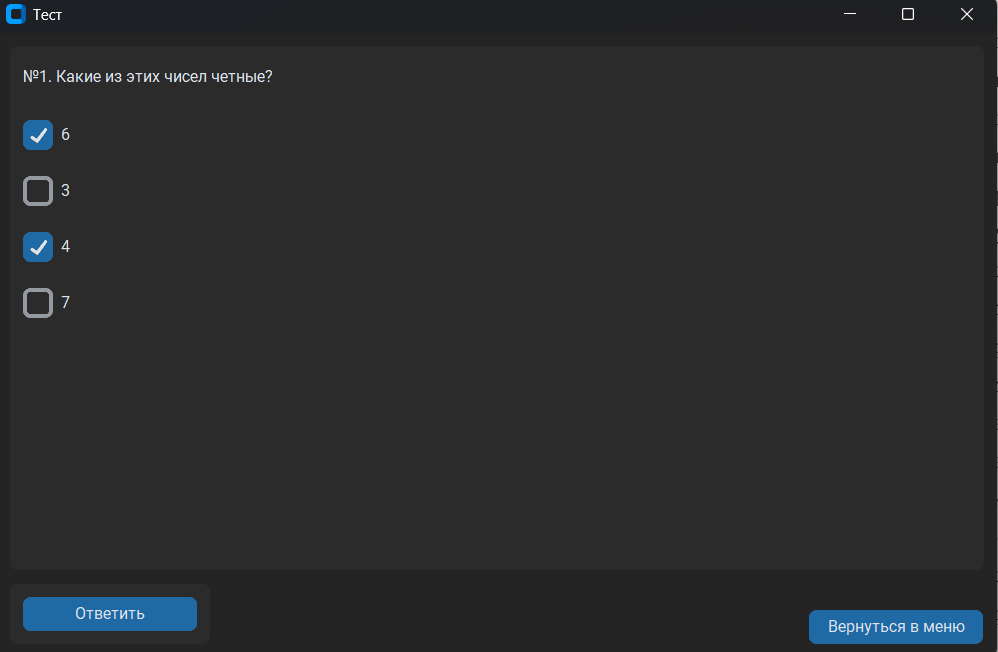
\includegraphics[width=1\linewidth]{тест_1.png}
	\caption{Окно "<Тест">}
	\label{test_window:image}
\end{figure}

\paragraph{Вариант использования <<Просмотр результатов - Пользователь>>}

Заинтересованные лица и их требования: пользователь желает посмотреть все результаты своих пройденных тестов.
\newline Предусловие: открыто окно "<Меню пользователя">.
\newline Постусловие: открыто окно "Результаты", отображены все результаты пройденных тестов пользователя.
\newline Основной успешный сценарий:
\begin{enumerate}
	\item Пользователь переходит в окно "<Результаты">.
	\item Приложение отображает соответствующее окно, где в табличном виде отображает информацию о завершённых тестах пользователя (см. рисунок ~\ref{user_results:image}).
\end{enumerate}

\begin{figure}[H]
	\centering
	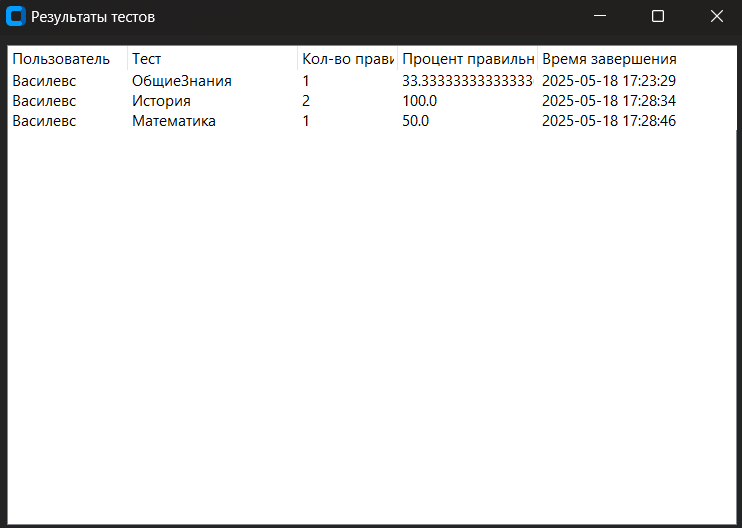
\includegraphics[width=1\linewidth]{результаты_пользователь.png}
	\caption{Окно "<Результаты">}
	\label{user_results:image}
\end{figure}


\paragraph{Вариант использования <<Авторизация администратора>>}

Заинтересованные лица и их требования: администратор желает создать новый тест и добавить в него вопрос.
\newline Предусловие: открыто окно "<Авторизация пользователя">.
\newline Постусловие: Авторизация администратора успешно выполнена. Открыт доступ к "<Меню администратора">.
\newline Основной успешный сценарий:
\begin{enumerate}
	\item Администратор переходит в окно "<Авторизация администратора">.
	\item Приложение отображает окно с двумя кнопками: "<Создать новый тест"> и "<Копировать текущий"> (см. рисунок ~\ref{admin_auth_window:image}).
	\item Администратор вводит пароль и нажимает кнопку "<Перейти в меню"> (см. рисунок ~\ref{admin_password:image}).
	\item Приложение проверяет введённый пароль, сообщает администратору об ошибке, если пароль неверный. Если пароль верный, открывает окно "<Меню администратора"> (см. рисунок ~\ref{admin_menu_1:image}).
\end{enumerate}

\begin{figure}[ht]
	\centering
	
\includegraphics[width=0.5\linewidth]{авторизация_администратора.png}
	\caption{Окно "<Авторизация администратора">}
	\label{admin_auth_window:image}
\end{figure}
\begin{figure}[H]
	\centering
	
\includegraphics[width=0.5\linewidth]{ввод_пароля_админ.png}
	\caption{Администратор вводит пароль}
	\label{admin_password:image}
\end{figure}
\begin{figure}[H]
	\centering
	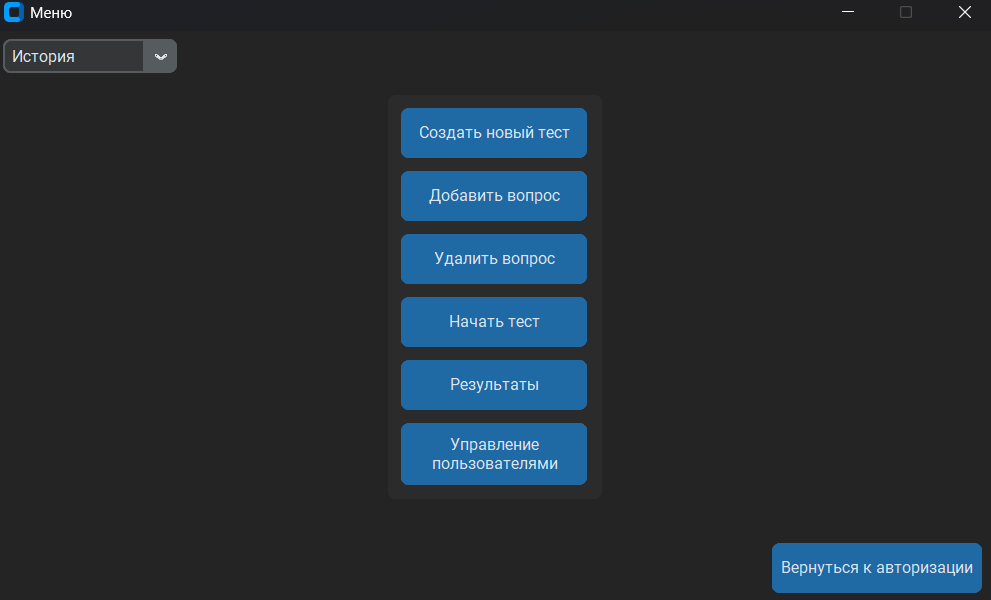
\includegraphics[width=1\linewidth]{меню_администратора.png}
	\caption{Окно "<Меню администратора">}
	\label{admin_menu_1:image}
\end{figure}

\paragraph{Вариант использования <<Изменение пароля администратора>>}

Заинтересованные лица и их требования: администратор желает свой изменить пароль.
\newline Предусловие: открыто окно "<Авторизация администратора">.
\newline Постусловие: Установлен новый пароль для авторизации администратора.
\newline Основной успешный сценарий:
\begin{enumerate}
	\item Администратор переходит в окно "<Изменение пароля">.
	\item Приложение отображает окно с тремя полями для ввода: старый пароль, новый пароль и повторение нового пароля. (см. рисунок ~\ref{admin_password_ch:image}).
	\item Администратор вводит старый пароль, два раза новый и нажимает кнопку "<Изменить пароль"> (см. рисунок ~\ref{admin_password_input:image}).
	\item Приложение проверяет старый пароль, новый пароль и его повтор, сообщает администратору об ошибке, если старый пароль неверный, или новый повторён неправильно, или новый пароль слишком простой. Если данные корректны, изменяет пароль и уведомляет администратора об успешном изменении пароля (см. рисунок ~\ref{admin_password_notif:image}).
\end{enumerate}

\begin{figure}[H]
	\centering
	
\includegraphics[width=0.6\linewidth]{изм_пароля_администратора.png}
	\caption{Окно "<Изменение пароля">}
	\label{admin_password_ch:image}
\end{figure}
\begin{figure}[H]
	\centering
	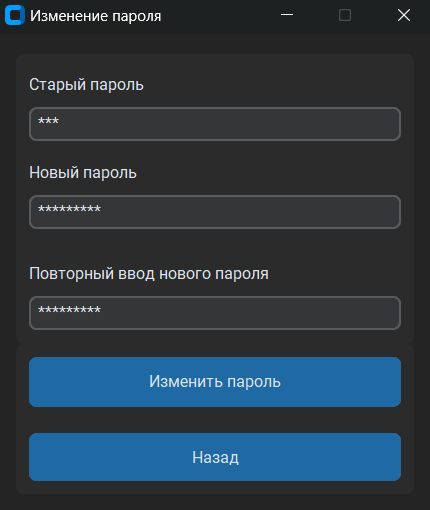
\includegraphics[width=0.6\linewidth]{изм_пар_адм_ввод.png}
	\caption{Ввод старого и нового паролей}
	\label{admin_password_input:image}
\end{figure}
\begin{figure}[H]
	\centering
	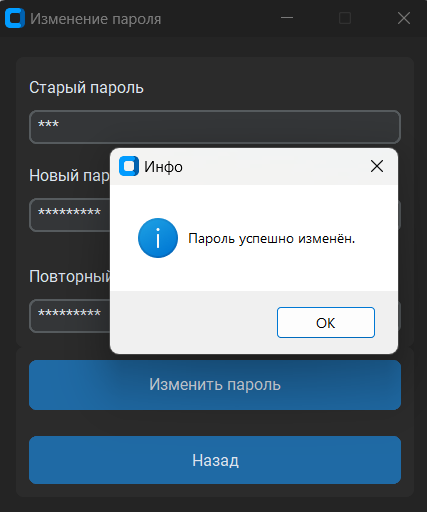
\includegraphics[width=0.6\linewidth]{изм_пар_адм_уведомление.png}
	\caption{Уведомление об успешном изменении пароля}
	\label{admin_password_notif:image}
\end{figure}

\paragraph{Вариант использования <<Просмотр результатов - Администратор>>}

Заинтересованные лица и их требования: администратор желает посмотреть результаты всех пользователей, сформировать диаграмму лучших результатов и сохранить её.
\newline Предусловие: открыто окно "<Меню администратора">.
\newline Постусловие: открыто окно "Результаты", отображены результаты всех пользователей, сформирована диаграмма лучших результатов и сохранена.
\newline Основной успешный сценарий:
\begin{enumerate}
	\item Администратор переходит в окно "<Результаты">.
	\item Приложение отображает соответствующее окно, где в табличном виде отображает информацию о завершённых тестах всех пользователей (см. рисунок ~\ref{admin_results:image}).
	\item Администратор нажимает кнопку "<Диаграмма">, чтобы наглядно увидеть лучшие результаты.
	\item Приложение отображает диаграмму лучших результатов (см. рисунок ~\ref{results_chart:image}).
	\item Администратор нажимает кнопку сохранения диаграммы и в файловом диалоге выбирает место для сохранения (см. рисунок ~\ref{saving_chart:image}).
\end{enumerate}

\begin{figure}[H]
	\centering
	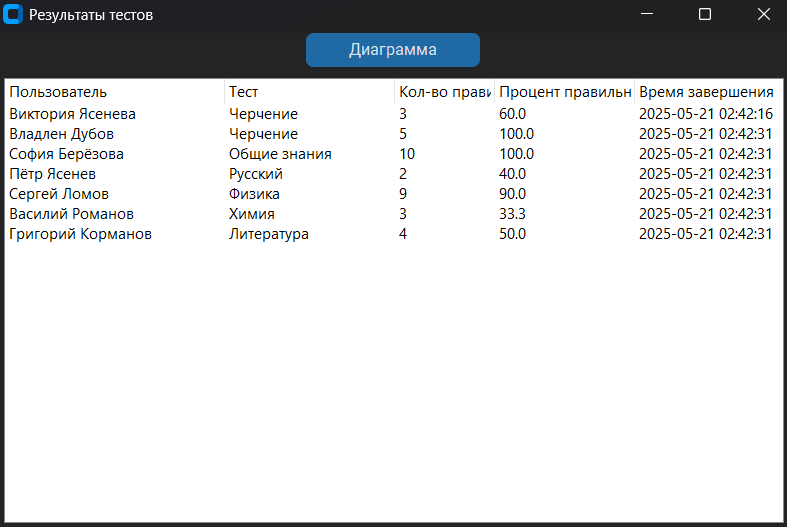
\includegraphics[width=1\linewidth]{результаты_админ.png}
	\caption{Окно "<Результаты">}
	\label{admin_results:image}
\end{figure}
\begin{figure}[H]
	\centering
	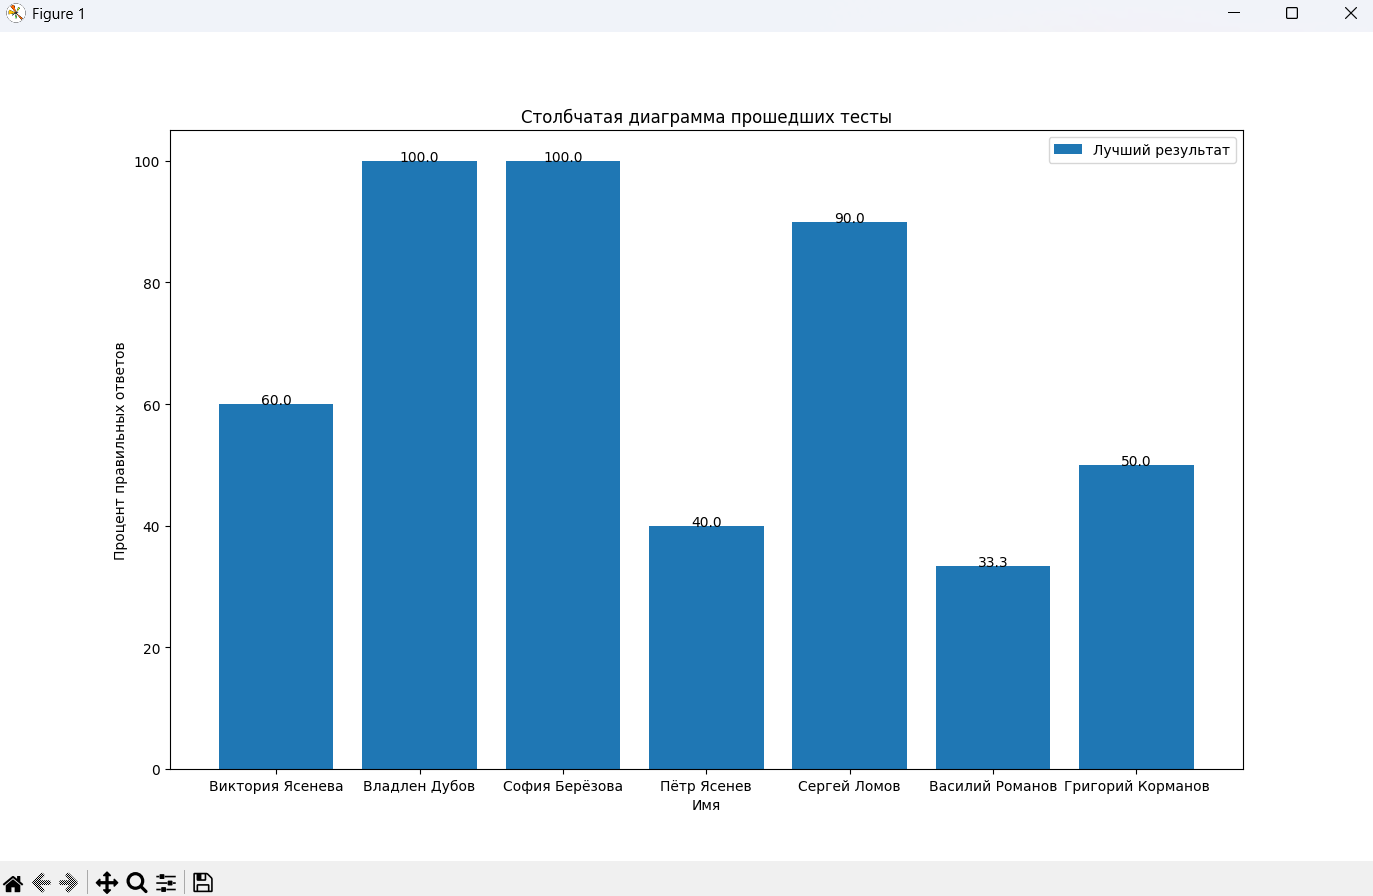
\includegraphics[width=1\linewidth]{результаты_диаграмма.png}
	\caption{Диаграмма результатов}
	\label{results_chart:image}
\end{figure}
\begin{figure}[H]
	\centering
	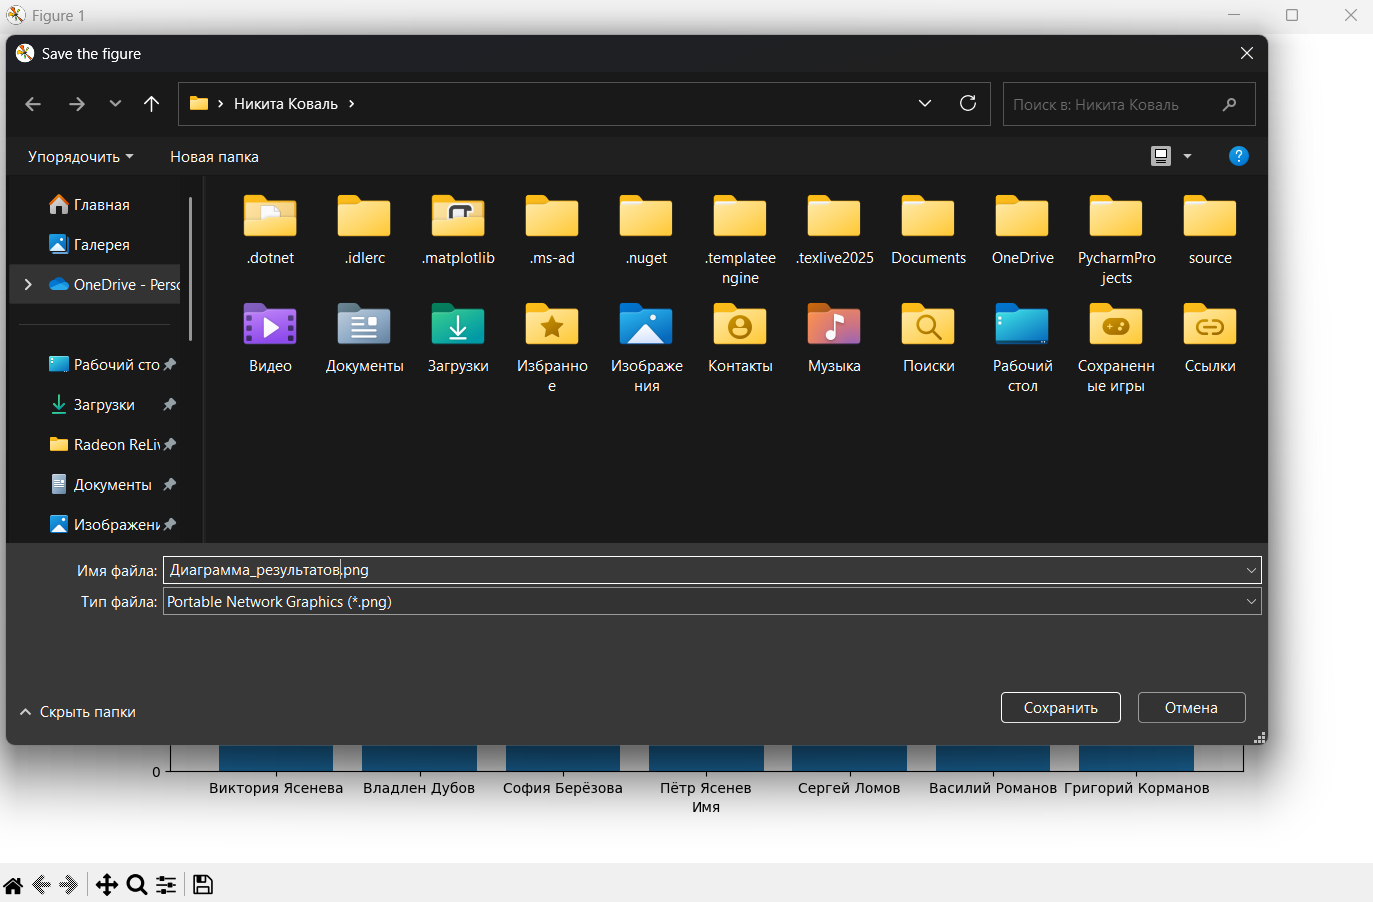
\includegraphics[width=1\linewidth]{сохранение_диаграммы_результатов.png}
	\caption{Диаграмма результатов}
	\label{saving_chart:image}
\end{figure}

\paragraph{Вариант использования <<Удаление вопроса>>}

Заинтересованные лица и их требования: администратор желает удалить вопрос из выбранного теста.
\newline Предусловие: открыто окно "<Меню администратора">.
\newline Постусловие: открыто окно "<Список вопросов">, отображены все вопросы выбранного теста, вопрос удалён.
\newline Основной успешный сценарий:
\begin{enumerate}
	\item Администратор выбирает тест, из которого хочет удалить вопрос (см. рисунок ~\ref{select_test:image}).
	\item Администратор переходит в окно "<Список вопросов">.
	\item Приложение отображает соответствующее окно, где отображены все вопросы выбранного теста (см. рисунок ~\ref{questions_window:image}).
	\item Администратор вводит номер удаляемого вопроса и нажимает кнопку "<Удалить вопрос"> (см. рисунок ~\ref{deleting_complete:image}).
	\item Приложение удаляет вопрос, обновляет список вопросов, сообщает администратору об успешном удалении вопроса и напоминает сохранить изменения (см. рисунок ~\ref{deleting_complete:image}).
	\item Администратор нажимает кнопку "<Сохранить изменения">.
	\item Приложение уведомляет администратора об успешном сохранении изменений (см. рисунок ~\ref{save_notification:image}).
\end{enumerate}

\begin{figure}[H]
	\centering
	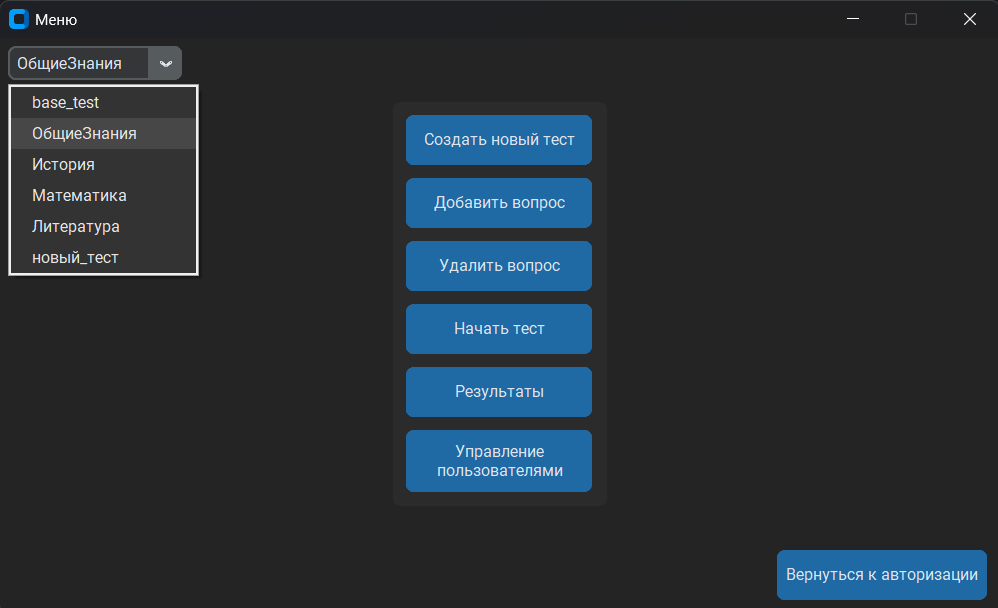
\includegraphics[width=1\linewidth]{выбор_теста.png}
	\caption{Выбор теста в окне "<Меню администратора">}
	\label{select_test:image}
\end{figure}
\begin{figure}[H]
	\centering
	
\includegraphics[width=1\linewidth]{вопросы.png}
	\caption{Окно "<Список вопросов">}
	\label{questions_window:image}
\end{figure}
\begin{figure}[H]
	\centering
	
\includegraphics[width=1\linewidth]{сообщение_об_удалении_вопроса.png}
	\caption{Уведомление об удалении вопроса}
	\label{deleting_complete:image}
\end{figure}
\begin{figure}[H]
	\centering
	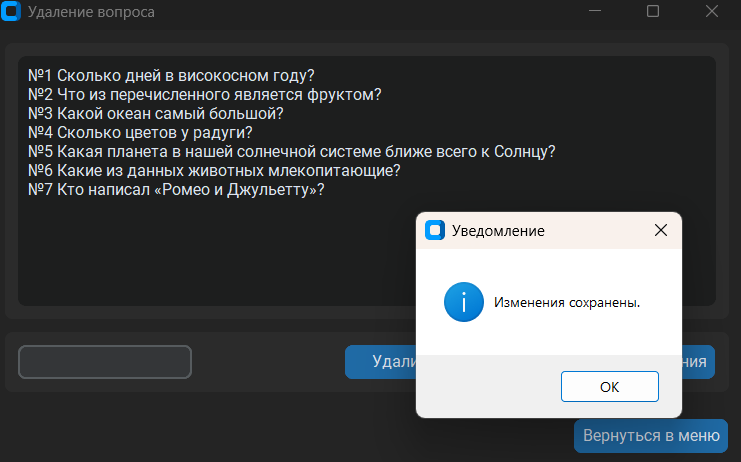
\includegraphics[width=1\linewidth]{сохранение_изменений_уд.png}
	\caption{Уведомление об успешном сохранении изменений}
	\label{save_notification:image}
\end{figure}

\paragraph{Вариант использования <<Создание пользователя администратором>>}

Заинтересованные лица и их требования: администратор желает добавить нового пользователя.
\newline Предусловие: открыто окно "<Меню администратора">.
\newline Постусловие: открыто окно "<Управление пользователями">, отображены все зарегистрированные пользователи, добавлен новый пользователь.
\newline Основной успешный сценарий:
\begin{enumerate}
	\item Администратор переходит в окно "<Управление пользователями">.
	\item Приложение отображает соответствующее окно, где отображены все зарегистрированные пользователи. (см. рисунок ~\ref{users:image}).
	\item Администратор нажимает кнопку "<Добавить пользователя">.
	\item Приложение отображает окно "<Создание пользователя"> (см. рисунок ~\ref{create_user:image}).
	\item Администратор заполняет имя и пароль нового пользователя и нажимает кнопку "<Создать"> (см. рисунок ~\ref{created_user:image}).
	\item Приложение уведомляет администратора об успешном создании нового пользователя (см. рисунок ~\ref{notification_user_created:image}).
\end{enumerate}

\begin{figure}[H]
	\centering
	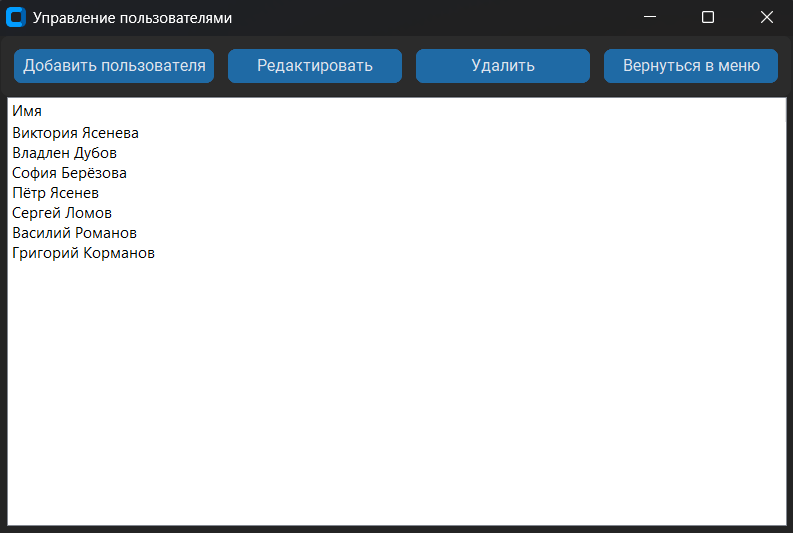
\includegraphics[width=1\linewidth]{управление_пользователями.png}
	\caption{Окне "<Управление пользователями">}
	\label{users:image}
\end{figure}
\begin{figure}[H]
	\centering
	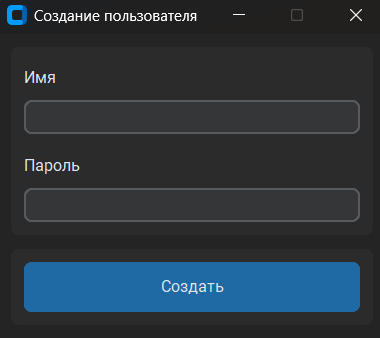
\includegraphics[width=0.6\linewidth]{создание_пользователя.png}
	\caption{Окне "<Создание пользователя">}
	\label{create_user:image}
\end{figure}
\begin{figure}[H]
	\centering
	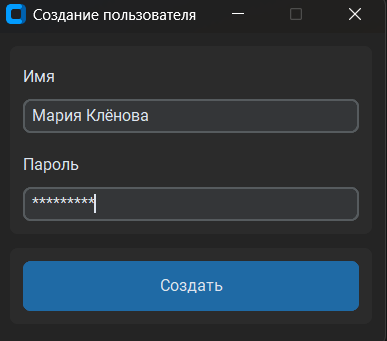
\includegraphics[width=0.6\linewidth]{соз_нов_пол_заполнено.png}
	\caption{Заполнение имени и пароля нового пользователя}
	\label{created_user:image}
\end{figure}
\begin{figure}[H]
	\centering
	
\includegraphics[width=0.6\linewidth]{пользователь_создан_уведомление.png}
	\caption{Уведомление об успешном создании нового пользователя}
	\label{notification_user_created:image}
\end{figure}

\paragraph{Вариант использования <<Удаление пользователя администратором>>}

Заинтересованные лица и их требования: администратор желает удалить пользователя.
\newline Предусловие: открыто окно "<Меню администратора">.
\newline Постусловие: открыто окно "<Управление пользователями">, отображены все зарегистрированные пользователи, пользователь удалён.
\newline Основной успешный сценарий:
\begin{enumerate}
	\item Администратор переходит в окно "<Управление пользователями">.
	\item Приложение отображает соответствующее окно, где отображены все зарегистрированные пользователи.
	\item Администратор выбирает пользователя, которого хочет удалить, и нажимает кнопку "<Удалить"> (см. рисунок ~\ref{deleting_user:image}).
	\item Приложение удаляет пользователя, обновляет список и уведомляет администратора об успешном удалении (см. рисунок ~\ref{user_deleted_notif:image}).
\end{enumerate}

\begin{figure}[H]
	\centering
	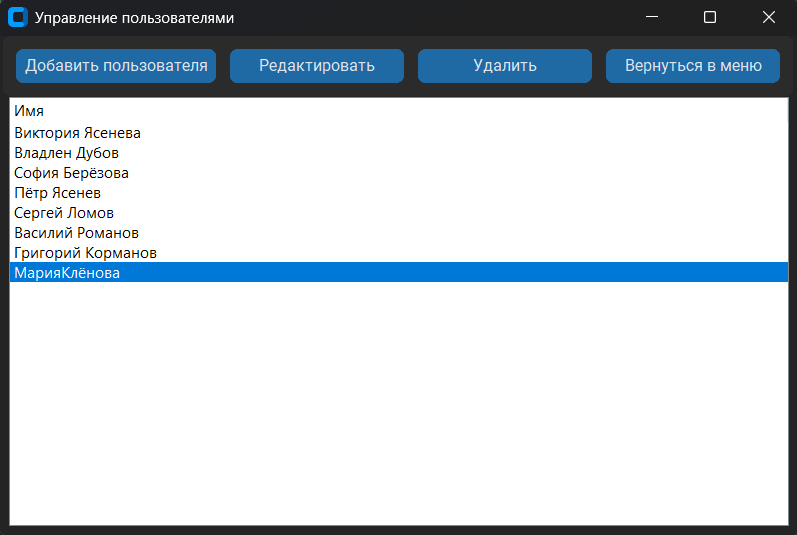
\includegraphics[width=1\linewidth]{удаление_пользователя.png}
	\caption{Удаление выбранного пользователя}
	\label{deleting_user:image}
\end{figure}
\begin{figure}[H]
	\centering
	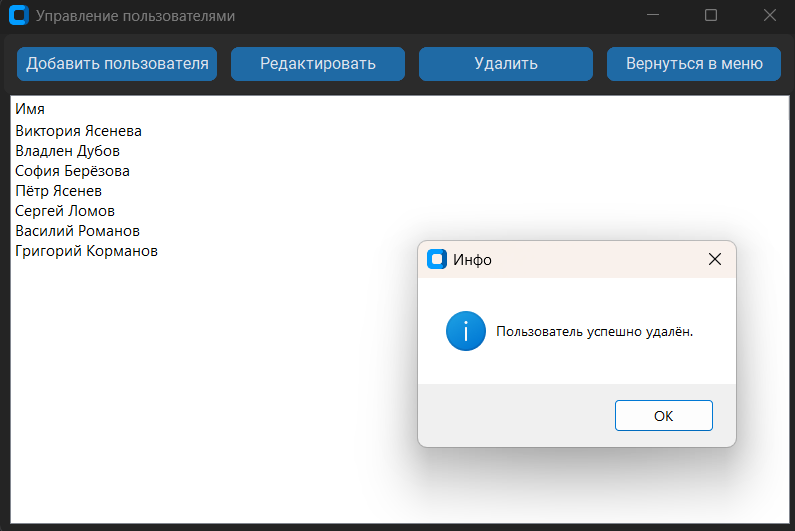
\includegraphics[width=1\linewidth]{пользователь_удалён.png}
	\caption{Уведомление об удалении пользователя}
	\label{user_deleted_notif:image}
\end{figure}

\paragraph{Вариант использования <<Редактирование пользователя администратором>>}

Заинтересованные лица и их требования: администратор желает редактировать пользователя.
\newline Предусловие: открыто окно "<Меню администратора">.
\newline Постусловие: открыто окно "<Управление пользователями">, отображены все зарегистрированные пользователи, изменены имя и пароль пользователя.
\newline Основной успешный сценарий:
\begin{enumerate}
	\item Администратор переходит в окно "<Управление пользователями">.
	\item Приложение отображает соответствующее окно, где отображены все зарегистрированные пользователи.
	\item Администратор выбирает пользователя, которого хочет отредактировать, и нажимает кнопку "<Редактировать"> (см. рисунок ~\ref{edit_user:image}).
	\item Приложение отображает окно с текущими данными пользователя, доступными для редактирования (см. рисунок ~\ref{edit_user_window:image}).
	\item Администратор изменяет имя и пароль пользователя, затем нажимает кнопку "<Сохранить изменения"> (см. рисунок ~\ref{edit_user_1:image}).
	\item Приложение сохраняет изменения, обновляет список пользователей и уведомляет администратора об изменении данных пользователя (см. рисунок ~\ref{edit_user_1:image}).
	\item Результат редактирования данных пользователя (см. рисунок ~\ref{edit_user_2:image})
\end{enumerate}

\begin{figure}[H]
	\centering
	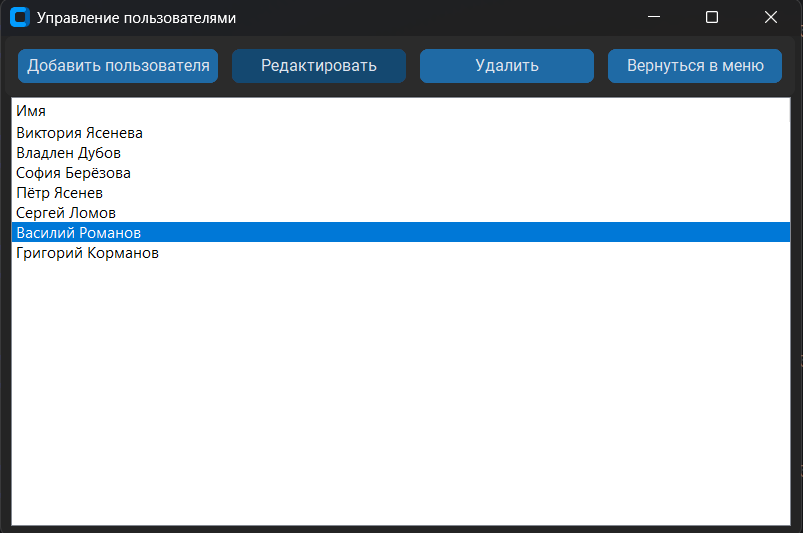
\includegraphics[width=1\linewidth]{ред_пользователя.png}
	\caption{Редактирование выбранного пользователя}
	\label{edit_user:image}
\end{figure}
\begin{figure}[H]
	\centering
	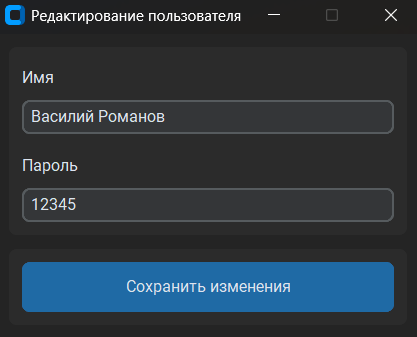
\includegraphics[width=0.6\linewidth]{ред_пол_окно.png}
	\caption{Окно "<Редактирование пользователя">}
	\label{edit_user_window:image}
\end{figure}
\begin{figure}[H]
	\centering
	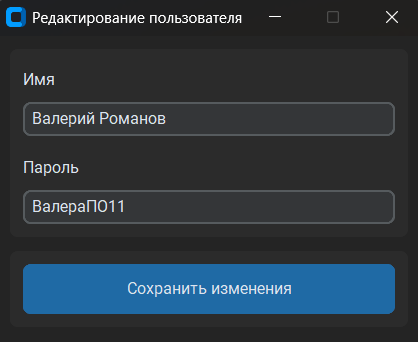
\includegraphics[width=0.6\linewidth]{ред_пол_1.png}
	\caption{Администратор меняет данные пользователя}
	\label{edit_user_1:image}
\end{figure}
\begin{figure}[H]
	\centering
	
\includegraphics[width=0.6\linewidth]{данные_изменены_ув.png}
	\caption{Уведомление об изменении данных пользователя}
	\label{edit_user_notif:image}
\end{figure}
\begin{figure}[H]
	\centering
	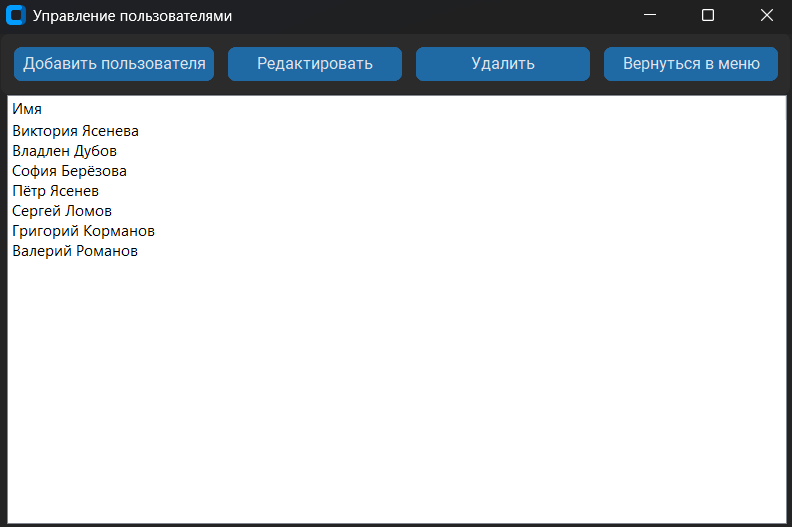
\includegraphics[width=1\linewidth]{изм_данных_пол_1.png}
	\caption{Результат редактирования данных}
	\label{edit_user_2:image}
\end{figure}

\paragraph{Вариант использования <<Создание нового теста и добавление в него вопроса с единственным выбором>>}

Заинтересованные лица и их требования: администратор желает создать новый тест и добавить в него вопрос.
\newline Предусловие: открыто окно "<Меню администратора">.
\newline Постусловие: Создан и сохранён новый тест с добавленным вопросом.
\newline Основной успешный сценарий:
\begin{enumerate}
	\item Администратор переходит в окно "<Создать тест">.
	\item Приложение отображает окно с двумя кнопками: "<Создать новый тест"> и "<Копировать текущий">.
	\item Администратор вводит имя нового теста и нажимает кнопку "<Создать новый тест"> (см. рисунок ~\ref{new_test_window:image}).
	\item Приложение оповещает администратора об успешном создании теста. 
	\item Администратор возвращается в меню, где выбирает созданный тест в выпадающем списке и нажимает кнопку "<Добавить вопрос"> (см. рисунок ~\ref{menu_new_test_window:image}).
	\item Приложение отображает окно "<Выбор типа вопроса"> с тремя кнопками: "<Вопрос с вводом">, "<Вопрос с единственным выбором"> и "<Вопрос с множественным выбором"> (см. рисунок ~\ref{question_selection:image}).
	\item Администратор нажимает кнопку добавить "<Вопрос с единственным выбором">.
	\item Приложение отображает окно для создания соответствующего вопроса.
	\item Администратор заполняет поле ввода для текста вопроса и переходит к созданию списка ответов: вводит ответ на вопрос и при помощи галочки в элементе интерфейса CheckBox указывает правильность ответа. В данном типе вопроса правильный ответ может быть только один. После чего нажимает кнопку "<Добавить ответ"> (см. рисунок ~\ref{radio_question:image}).
	\item Приложение отображает добавленный ответ и отмечает его зелёным цветом, если при создании он был выбран правильным.
	\item После добавления необходимого количества вопросов администратор нажимает кнопку "<Добавить вопрос">.
	\item Приложение добавляет вопрос с введённым текстом и созданным списком ответов в выбранный тест.
	\item Администратор нажимает кнопку "<Сохранить изменения">.
\end{enumerate}

\begin{figure}[H]
	\centering
	
\includegraphics[width=0.7\linewidth]{новый_тест.png}
	\caption{Окно "<Создание теста">}
	\label{new_test_window:image}
\end{figure}
\begin{figure}[H]
	\centering
	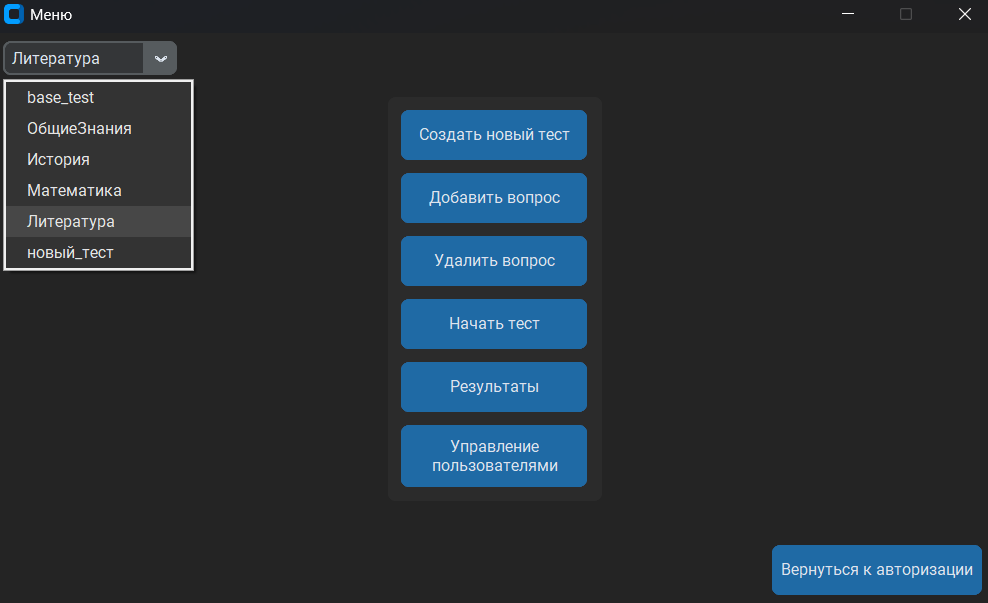
\includegraphics[width=1\linewidth]{меню_выбор_нового_теста.png}
	\caption{Выбор созданного теста в окне "<Меню администратора">}
	\label{menu_new_test_window:image}
\end{figure}
\begin{figure}[H]
	\centering
	
\includegraphics[width=0.6\linewidth]{выбор_типа_вопроса.png}
	\caption{Выбор типа создаваемого вопроса в окне "<Выбор типа вопроса">}
	\label{question_selection:image}
\end{figure}
\begin{figure}[H]
	\centering
	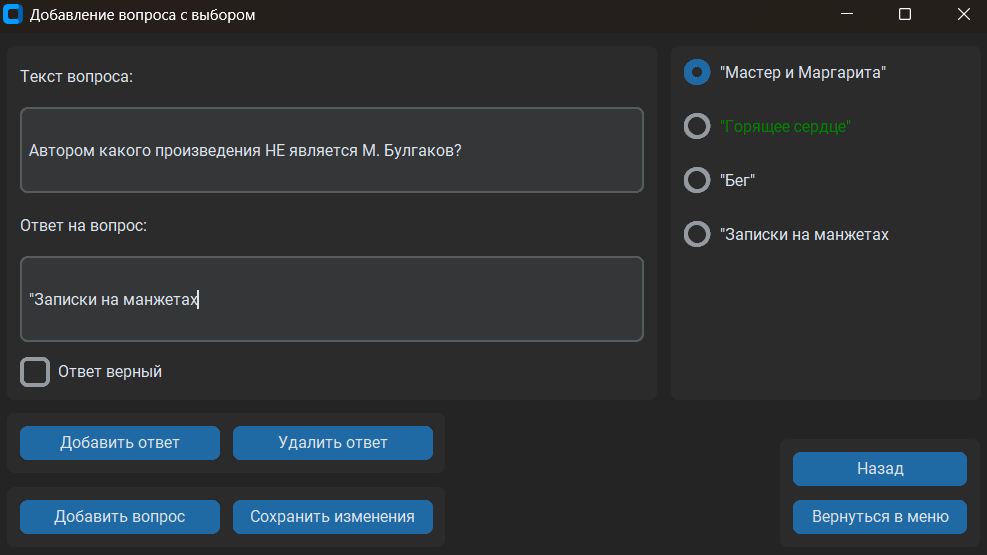
\includegraphics[width=1\linewidth]{добавление_вопроса_с_выбором.png}
	\caption{Окно "<Добавление вопроса с выбором">}
	\label{radio_question:image}
\end{figure}

\paragraph{Вариант использования <<Добавление нового вопроса с вводом ответа>>}

Заинтересованные лица и их требования: администратор желает добавить в тест новый вопрос с вводом ответа.
\newline Предусловие: открыто окно "<Меню администратора">.
\newline Постусловие: В выбранный администратором тест добавлен новый вопрос с вводом ответа.
\newline Основной успешный сценарий:
\begin{enumerate}
	\item Администратор выбирает желаемый тест в выпадающем списке и нажимает кнопку "<Добавить вопрос"> (см. рисунок ~\ref{select_test_1:image}).
	\item Приложение отображает окно "<Выбор типа вопроса"> с тремя кнопками: "<Вопрос с вводом ответа">, "<Вопрос с единственным выбором"> и "<Вопрос с множественным выбором"> (см. рисунок ~\ref{question_selection:image}).
	\item Администратор нажимает кнопку добавить "<Вопрос с вводом ответа">.
	\item Приложение отображает окно для создания соответствующего вопроса (см. рисунок ~\ref{adding_baseQuestion_window:image}).
	\item Администратор заполняет поле ввода для текста вопроса и поле ввода для ответа. После чего нажимает кнопку "<Добавить вопрос"> (см. рисунок ~\ref{adding_baseQuestion_1:image}).
	\item Приложение проверяет, что все поля заполнены, уведомляет администратора об успешном добавлении вопроса и напоминает сохранить изменения (см. рисунок ~\ref{adding_baseQuestion_2:image}).
	\item Администратор нажимает кнопку "<Сохранить изменения">.
	\item Приложение сохраняет изменения и выводит уведомление (см. рисунок ~\ref{adding_baseQuestion_3:image}).
\end{enumerate}

\begin{figure}[H]
	\centering
	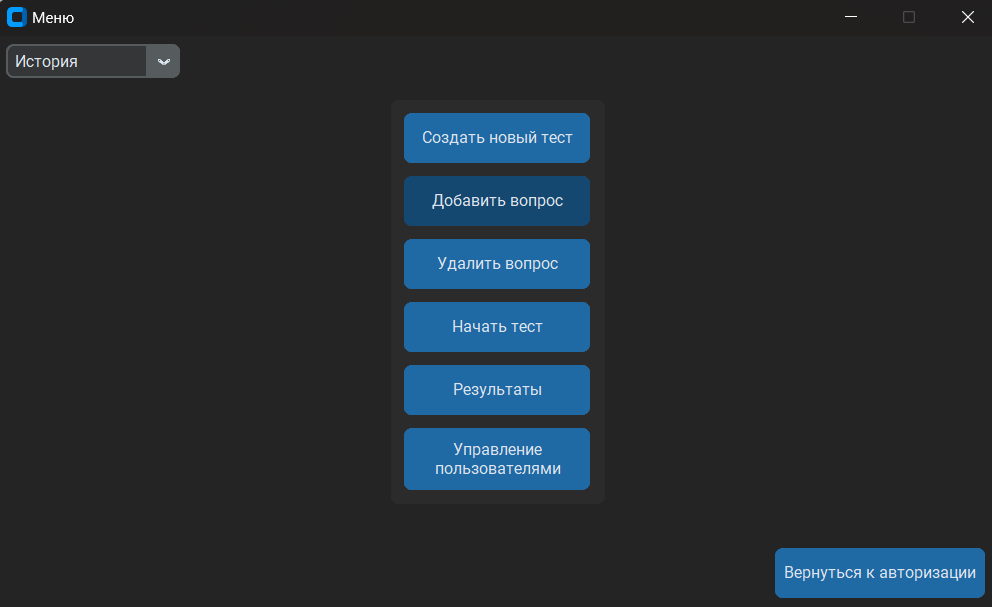
\includegraphics[width=1\linewidth]{выбор_теста_1.png}
	\caption{Выбор теста "<История"> и нажатие кнопки "<Добавить вопрос">}
	\label{select_test_1:image}
\end{figure}
\begin{figure}[H]
	\centering
	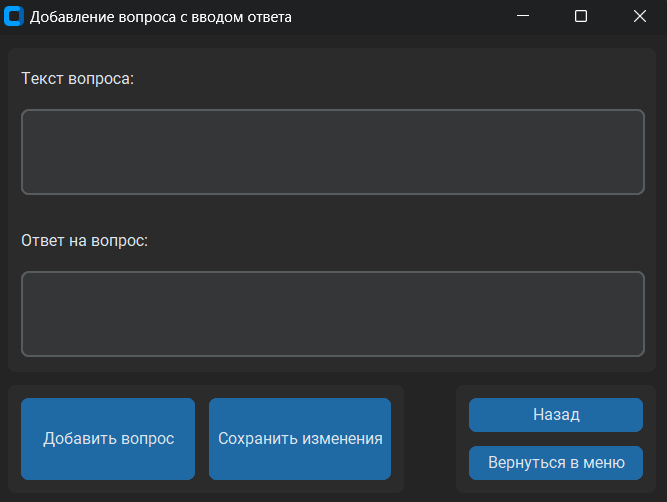
\includegraphics[width=0.6\linewidth]{доб_вопроса_с_вводом_окно.png}
	\caption{Окно "<Добавление вопроса с вводом ответа">}
	\label{adding_baseQuestion_window:image}
\end{figure}
\begin{figure}[H]
	\centering
	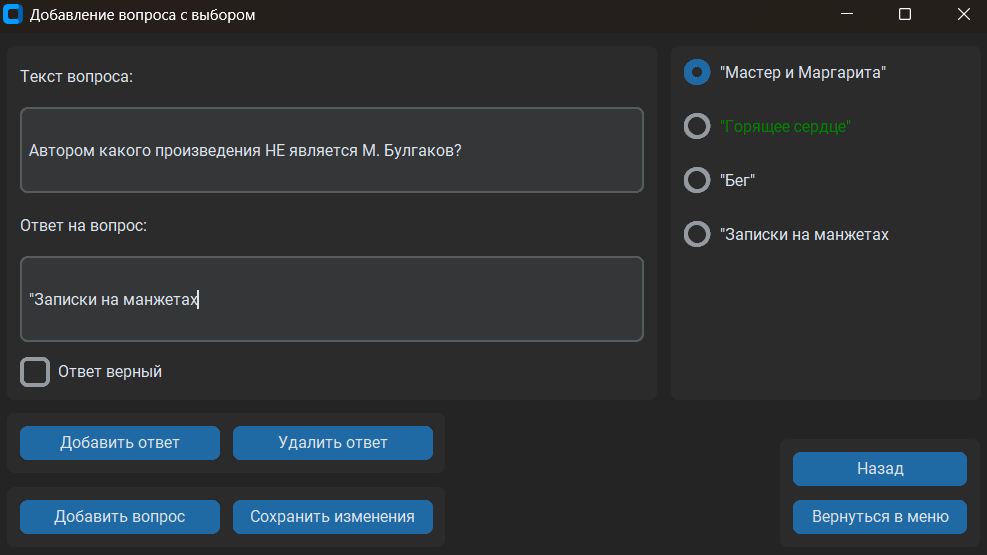
\includegraphics[width=1\linewidth]{добавление_вопроса_с_вводом_1.png}
	\caption{Ввод вопроса и ответа на него}
	\label{adding_baseQuestion_1:image}
\end{figure}
\begin{figure}[ht]
	\centering
	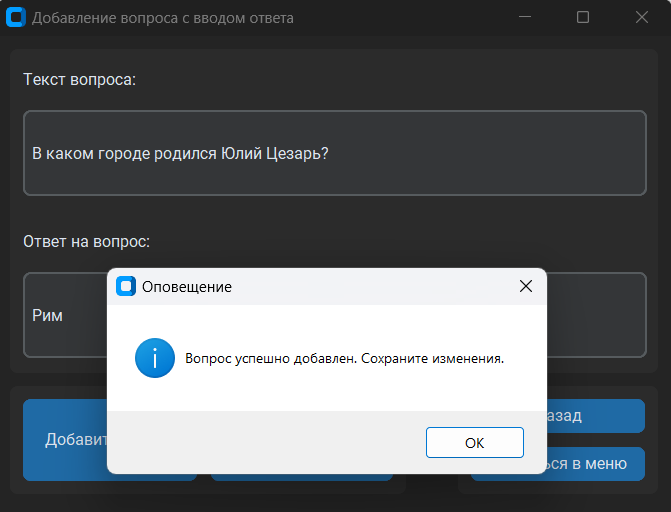
\includegraphics[width=1\linewidth]{доб_воп_ув_1.png}
	\caption{Уведомление об успешном добавлении вопроса}
	\label{adding_baseQuestion_2:image}
\end{figure}
\begin{figure}[H]
	\centering
	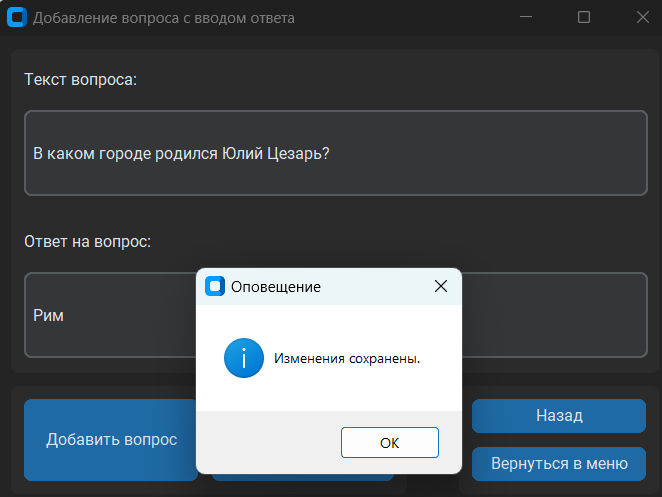
\includegraphics[width=1\linewidth]{уведомление_1.png}
	\caption{Уведомление о сохранении изменений}
	\label{adding_baseQuestion_3:image}
\end{figure}

\paragraph{Вариант использования <<Добавление нового вопроса с множественным выбором ответа>>}

Заинтересованные лица и их требования: администратор желает добавить в тест новый вопрос с множественным выбором ответа.
\newline Предусловие: открыто окно "<Меню администратора">.
\newline Постусловие: В выбранный администратором тест добавлен новый вопрос с множественным выбором ответа.
\newline Основной успешный сценарий:
\begin{enumerate}
	\item Администратор выбирает желаемый тест в выпадающем списке и нажимает кнопку "<Добавить вопрос">.
	\item Приложение отображает окно "<Выбор типа вопроса"> с тремя кнопками: "<Вопрос с вводом ответа">, "<Вопрос с единственным выбором"> и "<Вопрос с множественным выбором"> (см. рисунок ~\ref{question_selection:image}).
	\item Администратор нажимает кнопку добавить "<Вопрос с множественным выбором">.
	\item Приложение отображает окно для создания соответствующего вопроса (см. рисунок ~\ref{question_2:image}).
	\item Администратор заполняет поле ввода для текста вопроса и переходит к созданию списка ответов: вводит ответ на вопрос и при помощи галочки в элементе интерфейса CheckBox указывает правильность ответа. В данном типе вопроса правильных ответов может быть несколько. После чего нажимает кнопку "<Добавить ответ">.
	\item Приложение отображает добавленный ответ и отмечает его зелёным цветом, если при создании он был выбран правильным (см. рисунок ~\ref{question_input:image}).
	\item После добавления необходимого количества вопросов администратор нажимает кнопку "<Добавить вопрос">.
	\item Приложение проверяет, что все поля заполнены, уведомляет администратора об успешном добавлении вопроса и напоминает сохранить изменения (см. рисунок ~\ref{question_3t:image}).
	\item Администратор нажимает кнопку "<Сохранить изменения">.
	\item Приложение сохраняет изменения и выводит уведомление (см. рисунок ~\ref{question_4t:image}).
\end{enumerate}

\begin{figure}[H]
	\centering
	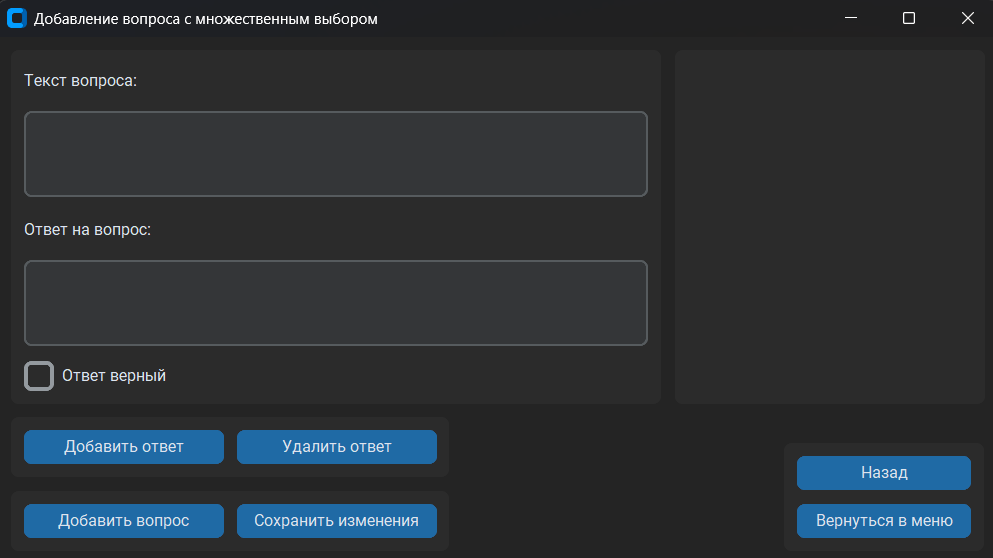
\includegraphics[width=1\linewidth]{вопрос_с_мн_выб.png}
	\caption{Окно "<Добавление вопроса с множественным выбором">}
	\label{question_2:image}
\end{figure}
\begin{figure}[H]
	\centering
	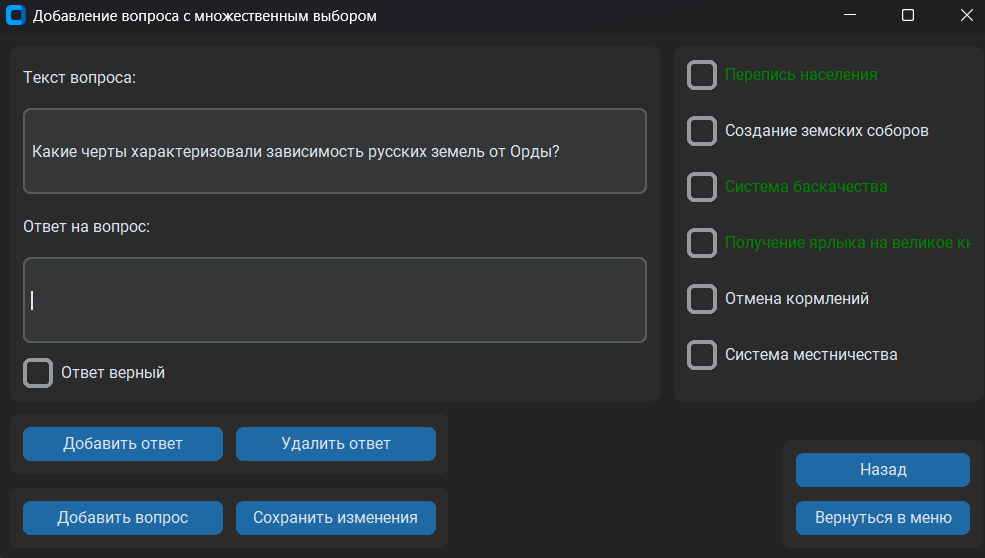
\includegraphics[width=1\linewidth]{ввод_вопроса_с_мн_выб.png}
	\caption{Ввод вопроса с множественным выбором}
	\label{question_input:image}
\end{figure}
\begin{figure}[H]
	\centering
	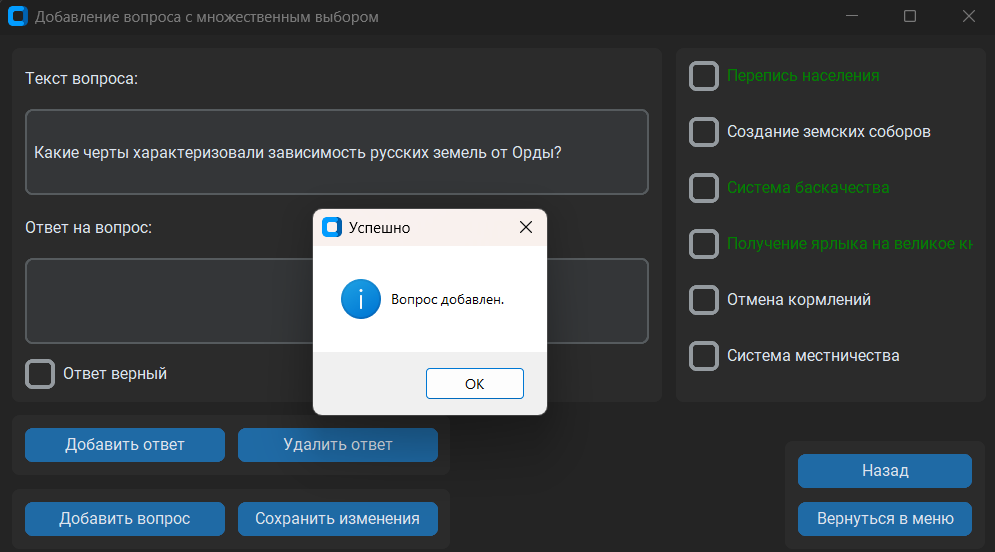
\includegraphics[width=1\linewidth]{доб_вопроса_с_мн_выбором.png}
	\caption{Уведомление о добавлении вопроса}
	\label{question_3t:image}
\end{figure}
\begin{figure}[H]
	\centering
	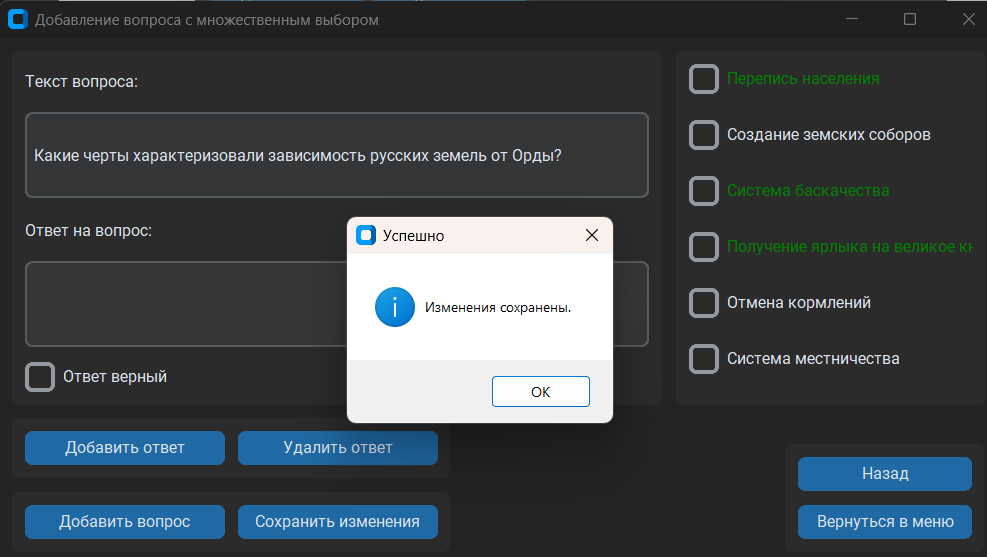
\includegraphics[width=1\linewidth]{доб_воп_3.png}
	\caption{Уведомление о сохранении изменений}
	\label{question_4t:image}
\end{figure}

\subsection{Требования пользователя к интерфейсу приложения}

Приложение должно иметь следующие основные экраны:
\begin{enumerate}
	\item Окно "<Авторизация"> - экран при открытии приложения, где пользователь может ввести имя и пароль для входа в свой аккаунт. Имеет переход в окна: "<Меню пользователя">, "<Регистрация">,  и "<Авторизоваться как администратор">.
	\item Окно "<Регистрация"> - экран приложения, на котором пользователь может зарегистрироваться. Имеет переход в окно "<Авторизация">.
	\item Окно "<Авторизоваться как администратор"> - экран приложения, на котором требуется ввести пароль администратора. После успешного ввода пароля позволяет перейти в специальное меню администратора с расширенными возможностями. Имеет переход в окна: "<Меню администратора">, "<Изменить пароль администратора"> и "<Вернуться к авторизации пользователя">.
	\item Окно "<Изменить пароль администратора"> - экран приложения, на котором пользователь может изменить пароль администратора, требуется ввести старый пароль и два раза новый. Имеет переход к окну "<Авторизоваться как администратор">.
	\item Окно "<Меню пользователя"> - экран приложения, на котором пользователь может выбрать тест и перейти к его прохождению, просмотреть результаты своих завершённых тестов. Имеет переходы в окна: "<Тест">, "<Результаты">.
	\item Окно "<Тест"> - экран приложения, на котором динамически отображаются вопросы теста и требуется ввести или выбрать соответствующий ответ.
	\item Окно "<Результаты"> - экран приложения, на котором в зависимости от прав доступа отображаются результаты пройденных тестов. Для пользователя отображаются только собственные результаты, для администратора - результаты всех пользователей с возможностью создания и выгрузки диаграммы, отображающей лучшие попытки прохождения тестов.
	\item Окно "<Меню администратора"> - экран приложения, на котором доступны все возможности системы тестирования знаний: создание и редактирование тестов, управление пользователями, просмотр и прохождение тестов, результаты тестов всех пользователей. Имеет переходы в окна: "<Создать тест">, "<Добавить вопрос">, "<Список вопросов">, "<Тест">, "<Управление пользователями">, "<Результаты">.
	\item Окно "<Создать тест"> - экран приложения, на котором можно создать новый тест с пустым списком вопросов или копировать список вопросов из выбранного теста. 
	\item Окно "<Добавление вопрос"> - экран приложения, на котором можно добавить три типа вопроса: с вводом ответа, с единственным выбором ответа, с множественным выбором.
	\item Окно "<Удаление вопроса"> - экран приложения, на котором отображен список всех вопросов теста с возможностью удаления любого вопроса из списка.
	\item Окно "<Управление пользователями"> - экран приложения, на котором отображены все зарегистрированные пользователи. Позволяет администратору добавлять, удалять и редактировать пользователей.
\end{enumerate}

\subsection{Требования к оформлению документации}

Разработка программной документации и программного изделия должна производиться согласно ГОСТ 19.102-77 и ГОСТ 34.601-90. Единая система программной документации.

\section{Технический проект}
\subsection{Общая характеристика организации решения задачи}

Необходимо спроектировать и разработать систему тестирования для контроля и оценки знаний.

Система тестирования представляет собой набор взаимосвязанных окон, содержащих текстовую и графическую информацию, которые сгруппированы по разделам. 

\subsection{Обоснование выбора технологии проектирования}

На сегодняшний день информационный рынок, поставляющий программные решения в выбранной сфере, предлагает множество продуктов, позволяющих достигнуть поставленной цели – разработки системы тестирования.

\subsubsection{Описание используемых технологий и языков программирования}

В процессе разработки системы тестирования используются программные средства и язык программирования. Каждое программное средство и язык программирования применяется для круга задач, при решении которых они необходимы.

\subsubsection{Язык программирования Python}

Python — это язык программирования, который широко используется в интернет-приложениях, разработке программного обеспечения, науке о данных и машинном обучении (ML). Разработчики используют Python, потому что он эффективен, прост в изучении и работает на разных платформах.

\subsubsection{Библиотека Tkinter}
Tkinter — это кроссплатформенный графический интерфейс Python, позволяющий работать с библиотекой Tk. Он содержит элементы графического интерфейса пользователя (GUI — Graphical User Interface), с помощью которых можно создавать различные приложения.

\paragraph{Достоинства языка Python}

К плюсам Python относятся: Простота. Его часто советуют в качестве первого “базового” языка, так как он очень прост в изучении и исполнении. В процессе написания программы не требуется использование фигурных скобок, как в других языках, что позволяет не отвлекаться на переключение между клавишами уделять больше внимания разработке программы. Обширность применения.

\paragraph{Недостатки языка Python}

Низкая скорость выполнения (причины: интерпретация, динамическая типизация) по сравнению с Delphi, C/C++, C\#, Java.
Отсутствие библиотек для создания "родных" интерфейсов для Windows.

\paragraph{Сравнение языков разметки JSON и XML}

В таблице ~\ref{JSONvsXM:table} перечислены все достоинства и недостатки языков разметки JSON и XML.

\begin{xltabular}{\textwidth}{|c|X|X|}
	\caption{Сравнение языков разметки JSON и XML\label{JSONvsXM:table}}\\ \hline
	~  & \centrow  JSON & \centrow XML \\ \hline
	\endfirsthead
	\continuecaption{Продолжение таблицы \ref{JSONvsXM:table}}
	~ & \centrow JSON & \centrow XML \\ \hline 
	\finishhead
	Удобочитаемость кода & + & - \\ \hline 
	Простота создания  & + & + \\ \hline 
	Простота использования & + & - \\ \hline 
	Расширяемость & + & - \\ \hline
	Отладка и исправление ошибок & - & + \\ \hline
	Безопасность & - & + \\ \hline
	Описание & JSON (англ. JavaScript Object Notation) — формат обмена данными, легко читаем людьми, легко обрабатывается и генерируется программами. & XML - это язык разметки подобный HTML. Расшифровывается как (англ. Extensible Markup Language - Расширяемый Язык Разметки) и является рекомендацией сообщества W3C в качестве языка разметки общего назначения (W3C recommended).
\end{xltabular}

\subsection{Диаграмма компонентов и схема обмена данными между файлами}

Диаграмма компонентов описывает особенности физического представления разрабатываемой системы. Она позволяет определить архитектуру системы, установив зависимости между программными компонентами, в роли которых может выступать как исходный, так и исполняемый код. Основными графическими элементами диаграммы компонентов являются компоненты, интерфейсы, а также зависимости между ними. На рисунке \ref{system_template:image} изображена диаграмма компонентов для проектируемой системы. Она включает в себя сервер с операционной системой, на которой установлена система управления содержимым, включающая в себя интерфейс. Помимо этого на диаграмме изображен клиентский компьютер с операционной системой, на которой установлено приложение.

\begin{figure}[ht]
\center{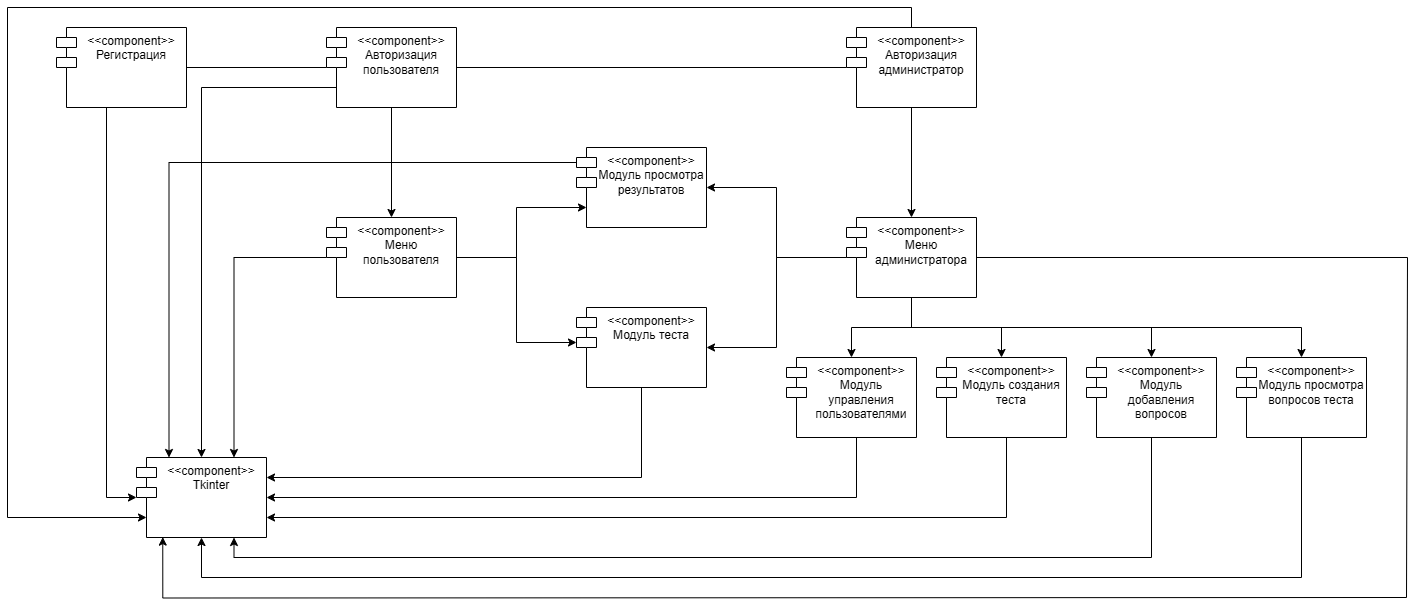
\includegraphics[width=1\linewidth]{диаграмма_компонентов.png}}
\caption{Диаграмма компонентов}
\label{system_template:image}
\end{figure}

Любой компонент должен быть вызван в сценарии окна системы тестирования. Окно передает данные компоненту в момент вызова последнего.

На рисунке \ref{exchange_scheme:image} представлена схема обмена данными между сценариями компонента при вызове компонента на текущем окне интерфейса.

\begin{figure}[H]
\center{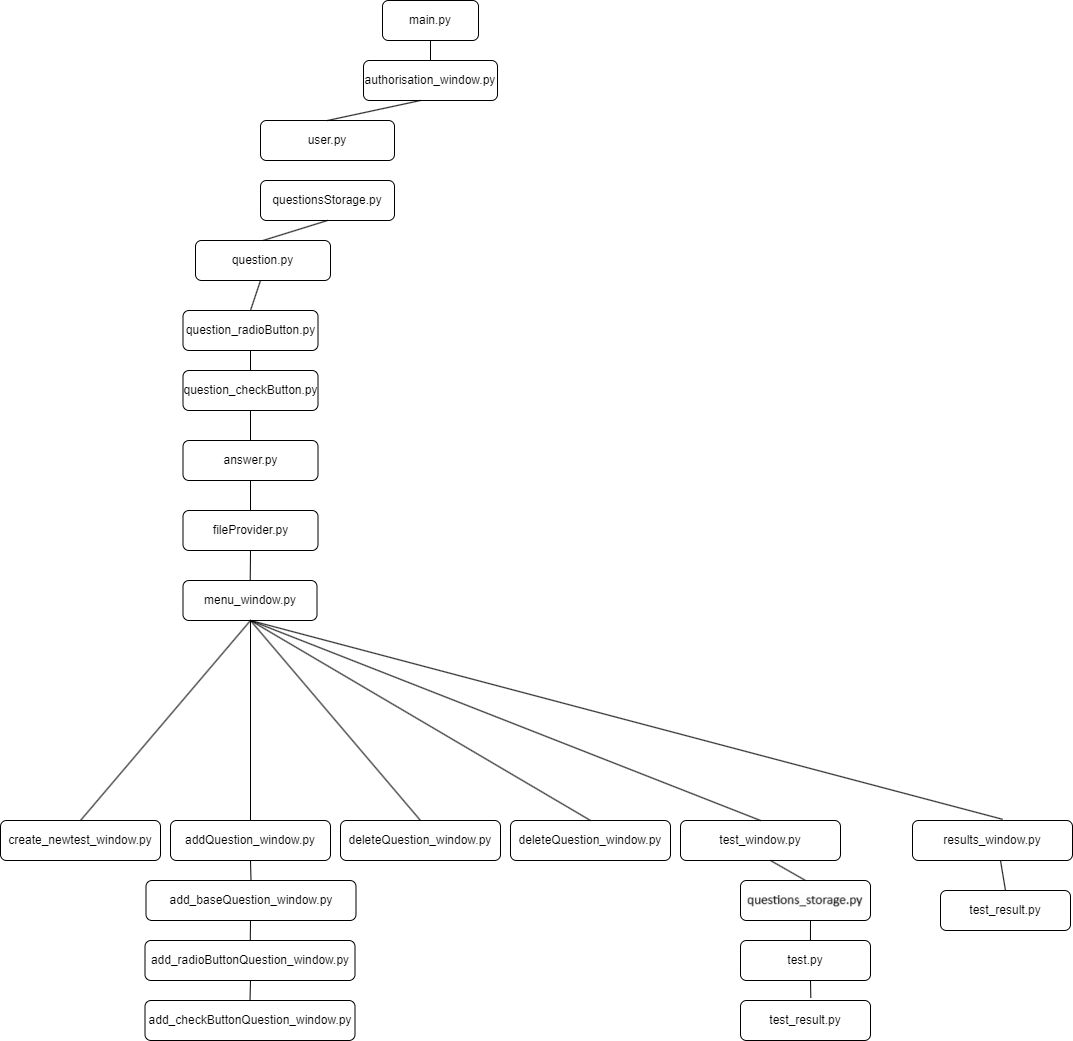
\includegraphics[width=0.8\linewidth]{exchange_scheme}}
\caption{Диаграмма зависимостей компонентов}
\label{exchange_scheme:image}
\end{figure}

При вызове компонента в сценарии системы тестирования указывается значения имя пользователя и набор вопросов соответствующий выбранному тесту, которые далее посредством ссылок на объекты классов, описывающих данную информацию передаются в следующее окно.

В зависимости от типа вопроса инициализируется соответствующее отображение с вариантами ответа.

Работа компонента заканчивается в момент закрытия главного окна.

\subsection{Содержание информационных блоков. Основные классы}

Проанализировав требования, можно выделить пять основных классов:
\begin{itemize}
\item "<Пользователь">;
\item "<Вопрос">;
\item "<Ответ">;
\item "<Тест">;
\item "<Результат">;
\end{itemize}

В состав сущности "<Пользователь"> можно включить атрибуты, представленные в таблице \ref{user:table}.

\begin{xltabular}{\textwidth}{|l|l|p{1.7cm}|X|}
	\caption{Атрибуты класса "<Пользователь">\label{user:table}}\\ \hline
	\centrow Поле & \centrow Тип & \centrow Обяза\-тельное & \centrow Описание \\ \hline
	\thead{1} & \thead{2} & \centrow 3 & \centrow 4 \\ \hline
	\endfirsthead
	\thead{1} & \thead{2} & \centrow 3 & \centrow 4 \\ \hline
	\finishhead
	\ name & String & true & Имя пользователя
\end{xltabular}

В состав класса "<Вопрос"> можно включить атрибуты, представленные в таблице \ref{question:table}.

\begin{xltabular}{\textwidth}{|l|l|p{1.7cm}|X|}
	\caption{Атрибуты класса "<Вопрос">\label{question:table}}\\ \hline
	\centrow Поле & \centrow Тип & \centrow Обяза\-тельное & \centrow Описание \\ \hline
	\thead{1} & \thead{2} & \centrow 3 & \centrow 4 \\ \hline
	\endfirsthead
	\thead{1} & \thead{2} & \centrow 3 & \centrow 4 \\ \hline
	\finishhead
	\ text & String & true & Текст вопроса \\ \hline
	answers & List[Answer] & true & Список вопросов
\end{xltabular}

В состав класса "<Ответ"> можно включить атрибуты, представленные в таблице \ref{answer:table}.

\begin{xltabular}{\textwidth}{|l|l|p{1.7cm}|X|}
	\caption{Атрибуты класса "<Ответ">\label{answer:table}}\\ \hline
	\centrow Поле & \centrow Тип & \centrow Обяза\-тельное & \centrow Описание \\ \hline
	\thead{1} & \thead{2} & \centrow 3 & \centrow 4 \\ \hline
	\endfirsthead
	\thead{1} & \thead{2} & \centrow 3 & \centrow 4 \\ \hline
	\finishhead
	\ text & String & true & Текст ответа \\ \hline
	is correct & Bool & false & Корректность вопроса
\end{xltabular}

В состав класса "<Тест"> можно включить атрибуты, представленные в таблице \ref{test:table}.

\begin{xltabular}{\textwidth}{|l|l|p{1.7cm}|X|}
	\caption{Атрибуты класса "<Тест">\label{test:table}}\\ \hline
	\centrow Поле & \centrow Тип & \centrow Обяза\-тельное & \centrow Описание \\ \hline
	\thead{1} & \thead{2} & \centrow 3 & \centrow 4 \\ \hline
	\endfirsthead
	\thead{1} & \thead{2} & \centrow 3 & \centrow 4 \\ \hline
	\finishhead
	\ name & String & true & имя теста \\ \hline
	questions & List[Question] & true & Список вопросов \\ \hline
	score & Integer & false & Счёт \\ \hline
	is started & Bool & false & Состояние теста \\ \hline
	current question id & Integer & false & ID текущего вопроса \\ \hline
	current answers & List[Answer] & false & Список ответов текущего вопроса
\end{xltabular}

В состав класса "<Результат"> можно включить атрибуты, представленные в таблице \ref{result:table}.

\begin{xltabular}{\textwidth}{|l|l|p{1.7cm}|X|}
	\caption{Атрибуты класса "<Результат">\label{result:table}}\\ \hline
	\centrow Поле & \centrow Тип & \centrow Обяза\-тельное & \centrow Описание \\ \hline
	\thead{1} & \thead{2} & \centrow 3 & \centrow 4 \\ \hline
	\endfirsthead
	\thead{1} & \thead{2} & \centrow 3 & \centrow 4 \\ \hline
	\finishhead
	\ user & User & true & Пользователь \\ \hline
	right answers count & Integer & true & Количество правильных ответов \\ \hline
	completion time & datetime & false & Время завершения теста
\end{xltabular}

В системе предусмотрен внутренний механизм связи между разделами и элементами информационных блоков, поэтому введения дополнительных идентификаторов при реализации связей между сущностями не предполагается.

Экземпляры сущностей реализуются в информационных блоках посредством элементов, атрибуты сущности – посредством полей и свойств элемента. 

\subsection{Проектирование пользовательского интерфейса}

На основании требований к пользовательскому интерфейсу, представленных в пункте 2.6 технического задания, был разработан графический интерфейс десктопного приложения. Для создания пользовательского
интерфейса используется библиотека Custom Tkinter.
На рисунке ~\ref{user_auth:image} представлен макет интерфейса вкладки «Авторизация пользователя». Макет содержит следующие элементы:
\begin{enumerate}
	\item Текстовое поле для ввода имени пользователя.
	\item Текстовое поле для ввода пароля пользователя.
	\item Кнопка авторизации, проверяет введённые данные пользователя, если они верны открывает меню пользователя.
	\item Кнопка регистрации, открывает окно регистрации пользователя.
	\item Кнопка для авторизации администратора. 
\end{enumerate}

\begin{figure}[H]
	\center{\includegraphics[width=0.6\linewidth]{макет_авторизация_пользователя}}
	\caption{Макет авторизации пользователя}
	\label{user_auth:image}
\end{figure}

На рисунке ~\ref{admin_auth:image} представлен макет интерфейса вкладки «Авторизация администратора». Макет содержит следующие элементы:
\begin{enumerate}
	\item Текстовое неизменяемое поле с надписью "Администратор".
	\item Текстовое поле для ввода пароля администратора.
	\item Кнопка авторизации, проверяет введённые данные пользователя, если они верны открывает меню администратора.
	\item Кнопка смены пароля администратора.
	\item Кнопка для авторизации пользователя. 
\end{enumerate}

\begin{figure}[H]
	\center{\includegraphics[width=0.6\linewidth]{макет_авторизация_админ}}
	\caption{Макет авторизации администратора}
	\label{admin_auth:image}
\end{figure}

На рисунке ~\ref{user_menu:image} представлен макет интерфейса вкладки «Меню пользователя». Макет содержит следующие элементы:
\begin{enumerate}
	\item Выпадающий список тестов для выбора.
	\item Кнопка запуска теста.
	\item Кнопка перехода к окну результатов пройденных тестов.
	\item Кнопка возврата к авторизации.
\end{enumerate}

\begin{figure}[H]
	\center{\includegraphics[width=1\linewidth]{макет_меню_пользователя}}
	\caption{Макет меню пользователя}
	\label{user_menu:image}
\end{figure}

На рисунке ~\ref{admin_menu:image} представлен макет интерфейса вкладки «Меню администратора». Макет содержит следующие элементы:
\begin{enumerate}
	\item Выпадающий список тестов для выбора.
	\item Кнопка создания нового теста.
	\item Кнопка добавления нового вопроса в выбранный тест.
	\item Кнопка перехода к окну со списком вопросов теста.
	\item Кнопка запуска теста.
	\item Кнопка просмотра результатов всех пользователей.
	\item Кнопка перехода в окно управления пользователями.
	\item Кнопка возврата к окну авторизации.
\end{enumerate}

\begin{figure}[H]
	\center{\includegraphics[width=1\linewidth]{макет_меню_админ}}
	\caption{Макет меню администратора}
	\label{admin_menu:image}
\end{figure}

\ifПрактика{}\else{
   \section{Рабочий проект}
\subsection{Классы, используемые при разработке сайта}

Можно выделить следующий список классов и их методов, использованных при разработке системы тестирования (таблица \ref{class:table}).

\renewcommand{\arraystretch}{0.8} % уменьшение расстояний до сетки таблицы
\begin{xltabular}{\textwidth}{|X|p{2.5cm}|>{\setlength{\baselineskip}{0.7\baselineskip}}p{4.85cm}|>{\setlength{\baselineskip}{0.7\baselineskip}}p{4.85cm}|}
\caption{Описание классов системы тестирования, используемых в приложении\label{class:table}}\\
\hline \centrow \setlength{\baselineskip}{0.7\baselineskip} Название класса & \centrow \setlength{\baselineskip}{0.7\baselineskip} Модуль, к которому относится класс & \centrow Описание класса & \centrow Методы \\
\hline \centrow 1 & \centrow 2 & \centrow 3 & \centrow 4\\ \hline
\endfirsthead
\caption*{Продолжение таблицы \ref{class:table}}\\
\hline \centrow 1 & \centrow 2 & \centrow 3 & \centrow 4\\ \hline
\finishhead
Test & Модуль теста & Test – класс, характеризующий тест и имеющий методы для его прохождения . & @propertydef get current question(self) - возвращает текущий вопрос, @property def get current answers(self) - возвращает ответы текущего вопроса,
def print current question(self) - возвращает номер вопроса и его текст,
@property def is finished(self) - возвращает статус завершения теста,
@staticmethod def shuffle(mas: []) - веремешивает переданный список и возвращает его,
def shuffle questions(self) - перемешивает вопросы текущего теста, ничего не возвращает,
def shuffle answers(self) - перемешивает ответы текущего вопроса, ничего не возвращает,
def start test(self) - запускает тест, обнуляет счёт и устанавливает id текущего вопроса, ничего не возвращает,
def next question(self) - делает инкремент id текущего вопроса и перемешивает его ответы, ничего не возвращает,
def accept answers(self, user answers: List[Answer]) - проверяет ответ на базовый вопрос и увеличивает счёт, если ответ правильный. Ничего не возвращает,
def  increase score(self) - увеличивает счёт, ничего не возвращает,
def summarise(self) - Возвращает диагноз соответствующий результату теста\\
\hline FileProvider & Модуль для работы с файловой системой & FileProvider – Класс для работы с файлами & @staticmethod def savetestresult(testresult: TestResult): Сохраняет переданный результат теста, ничего не возвращает, @staticmethod
def getresults(): Получает результаты тестов из файла, возвращает список результатов,  @staticmethod def cleartestresults(): Удаляет все результаты тестов,  @staticmethod def savetest(test: Test): Сохраняет переданные вопросы под переданным именем. Ничего не возвращает, @staticmethod def gettest(testpath: str): Получает тест по переданному пути, возвращает полученный тест, @staticmethod def savetestchanges(test: Test, testpath: str): Сохраняет переданные вопросы под переданным именем. Ничего не возвращает, @staticmethod def gettestnames(): Получает все сохранённые тесты, возвращает список названий тестов, @staticmethod def findtestpath(wantedtestname: str): Находит путь к тесту по его имени, возвращает путь.
\end{xltabular}
\renewcommand{\arraystretch}{1.0} % восстановление сетки

\subsection{Модульное тестирование разработанной системы тестирования}

Модульный тест для класса User из модели данных представлен на рисунке \ref{unitUser:image}.

\begin{figure}[ht]
\begin{lstlisting}[language=Python]
from django.test import TestCase
from .models import *
User = get_user_model()


class ShpoTestCases(TestCase):

    def setUp(self) -> None:
        self.user = User.objects.create(name="Gena")

    def test_2(self):

        self.assertEqual(self.user.name, 'Sad')
        print((self.user))
        print((self.user.name))
\end{lstlisting}  
\caption{Модульный тест класса User}
\label{unitUser:image}
\end{figure}

\subsection{Системное тестирование разработанной системы тестирования}

На рисунке \ref{authorisation:image} представлена авторизации в системе тестирования.
\begin{figure}[H] % H - рисунок обязательно здесь, или переносится, оставляя пустоту
\center{\includegraphics[width=1\linewidth]{authorisation}}
\caption{Авторизация в системе тестирования»}
\label{authorisation:image}
\end{figure}

На рисунке \ref{menu1:image} представлено меню.

\begin{figure}[H]
\center{\includegraphics[width=1\linewidth]{menu1}}
\caption{Меню}
\label{menu1:image}
\end{figure}

На рисунке \ref{test:image} представлено окно теста.

\begin{figure}[H]
\center{\includegraphics[width=1\linewidth]{test}}
\caption{Окно теста с одним из вопросов}
\label{test:image}
\end{figure}

   % !TeX spellcheck = ru_RU-Russian
\section*{ЗАКЛЮЧЕНИЕ}
\addcontentsline{toc}{section}{ЗАКЛЮЧЕНИЕ}

Разработанная система тестирования знаний представляет собой эффективное решение для автоматизации процесса оценки и контроля успеваемости. В ходе работы были успешно реализованы ключевые функции, такие как: создание и редактирование тестов, поддержка различных типов вопросов, автоматическая проверка ответов, формирование отчетов результатов, управление пользователями.

Система обладает рядом преимуществ, в числе которых: автоматизация, удобный интерфейс, объективность оценки, гибкость настройки. Система тестирования позволяет значительно сократить время на проверку работ, повысить объективность оценки, предоставить преподавателю отчёт о результатах всех пользователей.

В заключение, данная работа является успешным примером разработки современной системы тестирования знаний, отвечающей потребностям образовательного процесса и способствующей повышению его эффективности.

Основные результаты работы:

\begin{enumerate}
\item В ходе анализа предметной области были сформулированы основные цели и задачи систем тестирования знаний, изучены и описаны их основные компоненты, а также представлена история подобных систем с перечислением достоинств и недостатков каждого этапа развития.
\item Составление диаграмм компонентов и взаимодействия классов помогло визуализировать устройство разрабатываемой системы тестирования знаний, тем самым упростив понимание её архитектуры, выявить потенциальные проблемы на ранних этапах проектирования. Это позволило оптимизировать структуру системы, обеспечить её масштабируемость и упростить дальнейшую поддержку и развитие.
\item Описаны функциональные требования для создаваемого продукта. Определены требования к интерфейсу, входным и выходным данным.
\item Осуществлено проектирование приложения. Разработаны следующие модули приложения: модуль автоматической проверки ответов, модуль создания тестов, модуль редактирования тестов, модуль для управления пользователями. Разработан пользовательский интерфейс приложения для простого и удобного взаимодействия с программно-информационной системой для оценки и контроля  знаний.
\item Проведено модульное и системное тестирование приложения.
\end{enumerate}

Все требования, объявленные в техническом задании, были полностью реализованы, все задачи, поставленные в начале разработки проекта, были также решены.

Приложение находится в публичном доступе, поскольку опубликовано в сети Интернет.  

}\fi
\addcontentsline{toc}{section}{СПИСОК ИСПОЛЬЗОВАННЫХ ИСТОЧНИКОВ}

\begin{thebibliography}{9}

    \bibitem{javascript} Фримен, А. Практикум по программированию на JavaScript / А. Фримен. – Москва~: Вильямс, 2013. – 960 с. – ISBN 978-5-8459-1799-7. – Текст~: непосредственный.
    \bibitem{php} Бретт, М. PHP и MySQL. Исчерпывающее руководство / М. Бретт. – Санкт-Петербург : Питер, 2016. – 544 с. – ISBN 978-5-496-01049-8. – Текст~: непосредственный.
    \bibitem{css} Веру, Л. Секреты CSS. Идеальные решения ежедневных задач / Л. Веру. – Санкт-Петербург : Питер, 2016. – 336 с. – ISBN 978-5-496-02082-4. – Текст~: непосредственный.
    \bibitem{mysql}	Гизберт, Д. PHP и MySQL / Д. Гизберт. – Москва~: НТ Пресс, 2013. – 320 с. – ISBN 978-5-477-01174-2. – Текст~: непосредственный.
	\bibitem{html5}	Голдстайн, А. HTML5 и CSS3 для всех / А. Голдстайн, Л. Лазарис, Э. Уэйл. – Москва~: Вильямс, 2012. – 368 с. – ISBN 978-5-699-57580-0. – Текст~: непосредственный.
	\bibitem{htmlcss}	Дэкетт, Д. HTML и CSS. Разработка и создание веб-сайтов / Д. Дэкетт. – Москва~: Эксмо, 2014. – 480 с. – ISBN 978-5-699-64193-2. – Текст~: непосредственный.
	\bibitem{bigbook}	Макфарланд, Д. Большая книга CSS / Д. Макфарланд. – Санкт-Петербург : Питер, 2012. – 560 с. – ISBN 978-5-496-02080-0. – Текст~: непосредственный.
	\bibitem{uchiru}	Лоусон, Б. Изучаем HTML5. Библиотека специалиста / Б. Лоусон, Р. Шарп. – Санкт-Петербург : Питер, 2013 – 286 с. – ISBN 978-5-459-01156-2. – Текст~: непосредственный.
	\bibitem{chaynik}	Титтел, Э. HTML5 и CSS3 для чайников / Э. Титтел, К. Минник. – Москва~: Вильямс, 2016 – 400 с. – ISBN 978-1-118-65720-1. – Текст~: непосредственный.    
	\bibitem{22}	Титтел, Э. HTML5 и CSS3 для чайников / Э. Титтел, К. Минник. – Москва~: Вильямс, 2016 – 400 с. – ISBN 978-1-118-65720-1. – Текст~: непосредственный.    
	\bibitem{1231}	Титтел, Э. HTML5 и CSS3 для чайников / Э. Титтел, К. Минник. – Москва~: Вильямс, 2016 – 400 с. – ISBN 978-1-118-65720-1. – Текст~: непосредственный.    
	\bibitem{sdf}	Титтел, Э. HTML5 и CSS3 для чайников / Э. Титтел, К. Минник. – Москва~: Вильямс, 2016 – 400 с. – ISBN 978-1-118-65720-1. – Текст~: непосредственный.    
	\bibitem{servsssds}	Титтел, Э. HTML5 и CSS3 для чайников / Э. Титтел, К. Минник. – Москва~: Вильямс, 2016 – 400 с. – ISBN 978-1-118-65720-1. – Текст~: непосредственный.
\end{thebibliography}

\ifВКР{\appendix{Представление графического материала}

Графический материал, выполненный на отдельных листах,
изображен на рисунках А.1--А.\arabic{числоПлакатов}.
\setcounter{числоПлакатов}{0}

\renewcommand{\thefigure}{А.\arabic{figure}} % шаблон номера для плакатов

\begin{landscape}

\begin{плакат}
    \includegraphics[width=0.82\linewidth]{плакат1.png}
    \заголовок{Сведения о ВКРБ}
    \label{pl1:image}      
\end{плакат}

\begin{плакат}
    \includegraphics[width=0.82\linewidth]{плакат2.png}
    \заголовок{Цель и задачи разработки}
    \label{pl2:image}      
\end{плакат}

\begin{плакат}
    \includegraphics[width=0.82\linewidth]{плакат3.png}
    \заголовок{Концептуальная модель сайта}
    \label{pl3:image}      
\end{плакат}

\begin{плакат}
    \includegraphics[width=0.82\linewidth]{плакат3.png}
    \заголовок{Еще плакат}
    \label{pl4:image}      
\end{плакат}

\end{landscape}
}\fi
\ifПрактика{}\else{\appendix{Фрагменты исходного кода программы}

main.tex
\lstinputlisting[language=Tex, frame=none]{main.tex}

ТехПроект.tex
\lstinputlisting[language=Tex, frame=none]{ТехПроект.tex}

\ifВКР{
\newpage
\addcontentsline{toc}{section}{На отдельных листах (CD-RW в прикрепленном конверте)}
\begin{center}
\textbf{Место для диска}
\end{center}
}\fi
}\fi
\end{document}
